\documentclass[
germanthesis
]{i3thesis}
% options:
% [germanthesis] - Thesis is written in German
% [plainunnumbered] - Don't print numbers on plain pages
% [earlydraft] - Settings for quick draft printouts
% [watermark] - Print current time/date at bottom of each page
% [phdthesis] - switch to PhD thesis style
% [twoside] - double sided

\usepackage{multirow}
\usepackage{floatflt}
%\usepackage[babel=true]{csquotes}
%\usepackage[backend=biber,style=ieee]{biblatex}

%% CUSTOM
% ------------------------------
% for figures
\usepackage{caption}
\usepackage{subcaption}
\usepackage{tocloft}

% tables
\usepackage{longtable}
\usepackage{pdflscape}
\usepackage{xurl}
\usepackage{tabularx}
\usepackage{booktabs}
\usepackage{ragged2e}

% subchapters in capital
\newcommand{\sh}[1]{
  \vspace{1em}
  \noindent\MakeUppercase{#1}\\
}

% acronyms
\newcommand{\listofacronyms}{%
  \chapter*{\glossarytitlename}%
  \addcontentsline{toc}{chapter}{\glossarytitlename}%
  \begin{acronym}[XXXX]
  \end{acronym}%
}
% ------------------------------

\author{Dustin Heither}
\title{Best Practices und Trends bei didaktischen Simulatoren für Rechnerarchitektur:
Eine systematische Literaturrecherche}
\thesistype{Bachelorarbeit}
\thesiscite{Bachelor's Thesis~(Bachelorarbeit)}
\birthday{10. Mai 1992}
\birthplace{Oberhausen}
\thesisstart{30. April 2025}
\advisors{M.Sc. Tobias Baumeister}

\addbibresource{thesis.bib}
\graphicspath{{images/},{pictures/}}

\begin{document}
\pagenumbering{roman}

\maketitle
\begin{abstract}
Die vorliegende Bachelorarbeit untersucht systematisch den Einsatz didaktischer Simulatoren in der Lehre der Rechnerarchitektur. Ziel war es, relevante Simulatoren und wissenschaftliche Beiträge zu erfassen, anhand eines Kriterienkatalogs zu analysieren und daraus Best Practices sowie aktuelle Trends abzuleiten. Grundlage ist eine systematische Literaturrecherche in IEEE Xplore, ACM Digital Library und weiteren Quellen sowie eine ergänzende Erhebung veröffentlichter Simulatoren. Insgesamt wurden 151 Publikationen und 57 Simulatoren identifiziert und nach thematischen Clustern sowie didaktischen Merkmalen ausgewertet.  

Die Ergebnisse zeigen deutliche Schwerpunkte bei Prozessorarchitekturen, insbesondere im Kontext von \acs{RISC}, während GPUs, KI-gestützte Ansätze und immersive Technologien zunehmend an Bedeutung gewinnen. Didaktisch wirksam sind vor allem reduzierte Darstellungen nach Prinzipien der Cognitive Theory of Multimedia Learning (CTML). Erfolgsfaktoren sind eine kostenfreie, plattformübergreifende Verfügbarkeit und eine verlässliche Dokumentation. Gamification wird bislang selten umgesetzt, bietet jedoch Potenzial zur Steigerung der Motivation.  

Die Diskussion verdeutlicht, dass empirische Wirksamkeitsstudien unter realen Lehrbedingungen fehlen und der Kriterienkatalog ausgeweitet werden sollte.  

Das Fazit lautet, dass Simulatoren gezielt für kurze, klar strukturierte Lerneinheiten konzipiert und durch motivierende Elemente ergänzt werden sollten. Künftige Forschung sollte Feldstudien durchführen, objektive Qualitätsmaßstäbe entwickeln und den schulischen Bereich stärker berücksichtigen. Damit liefert die Arbeit sowohl konsolidierte Gestaltungsprinzipien für die Praxis als auch Impulse für die zukünftige Forschung.
\end{abstract}
\acresetall

\cleardoublepage
\tableofcontents

\cleardoublepage
\listofacronyms
\TODO{Alphabetisch sortieren}

\begin{acronym}[1234567890]
    \acro{FPGA}{Field Programmable Gate Array}
    \acro{OER}{Open Educational Resources}
    \acro{MOOC}{Massive Open Online Course}
    \acro{AR}{Augmented Reality}
    \acro{VR}{Virtual Reality}
    \acro{MR}{Mixed Reality}
    \acro{XR}{Extended Reality}
    \acro{CTML}{Cognitive Theory of Multimedia Learning}
    \acro{ELT}{Experiential Learning Theory}
    \acro{CISC}{Complex Instruction Set Computer}
    \acro{RISC}{Reduced Instruction Set Computer}
    \acro{ILP}{Instruction-Level Parallelsim}
    \acro{SMT}{Simultaneous Multithreading}
    \acro{SaaS}{Software as a Service}
    \acro{DLP}{Data-Level Parallelism}
    \acro{TLP}{Thread-Level Parallelism}
    \acro{DSA}{Domain-Specific Architectures}
    \acro{TPU}{Tensor Processing Unit}
    \acro{SIMD}{Single Instruction Multiple Data}
    \acro{NPU}{Neural Processing Unit}
    \acro{PDA}{Personal Digital Assistant}
    \acro{CAI}{Computer Assisted Instruction}
    \acro{LMS}{Learning Management Systems}
    \acro{LXP}{Learning Experience Platforms}
    \acro{BMBF}{Bundesministerium für Bildung und Forschung}
    \acro{OS}{Operating System}
    \acro{AI}{Artificial Intelligence}
\end{acronym}


\cleardoublepage
\pagenumbering{arabic}

\chapter{Einleitung}

\section{Motivation}

Die nachfolgende Bachelorarbeit behandelt das Thema "Best Practices und Trends bei didaktischen Simulatoren für Rechnerarchitektur: Eine systematische Literaturrecherche". Sie wurde am Lehrstuhl für Rechnerarchitektur der Universität Erlangen-Nürnberg im Sommersemester 2025 geschrieben und bildet die abschließende Prüfungsleistung des Bachelorstudiums Informatik.



\section{Zielsetzung}

Innerhalb dieser Arbeit werden Simulatoren vorgestellt und untersucht, die Relevanz in den Themengebieten der Rechnerarchitektur haben und für didaktische Zwecke genutzt werden.

\section{Aufbau der Arbeit}

\chapter{Methodik}

\section{Recherche und Auswahl der Simulatoren}

\section{Kriterienkatalog}

Tabelle~\ref{tab:kriterien} fasst die für die Analyse herangezogenen Kriterien zusammen.

Ein zentrales Kriterium ist der \textit{Zugriff}. Je nach organisatorischem Kontext ist entscheidend, ob ein Simulator online oder offline verfügbar ist. Während eine Online-Lösung eine Internetverbindung erfordert und dadurch eingeschränkt nutzbar sein kann, setzt ein Offline-Simulator häufig eine Installation voraus, die wiederum von Betriebssystem oder Hardwareanforderungen abhängt.

Die \textit{Programmiersprache} ist insbesondere für Studierende der Informatik von Relevanz. Sie kann die Möglichkeit eröffnen, Erweiterungen oder Plugins zu entwickeln und den Simulator an spezifische Bedürfnisse anzupassen.

Unter dem Kriterium \textit{Simulatorart} wird der Abstraktionsgrad eingeordnet, also ob der Simulator didaktisch reduziert oder realitätsnah ist. Ergänzend werden auch die Visualisierung und der Grad der Interaktivität berücksichtigt.

Das Kriterium \textit{Zielgruppe} erlaubt eine Zuordnung zu unterschiedlichen Bildungskontexten (z. B. Schule, Hochschule) und gibt Auskunft darüber, ob und in welchem Umfang Vorkenntnisse erforderlich sind.

Für Lehrende spielt zudem der \textit{Preis} eine zentrale Rolle. Es wird unterschieden, ob es sich um freie oder lizenzpflichtige Software handelt, da der Kostenfaktor maßgeblich über den praktischen Einsatz entscheidet.

Ein weiterer Aspekt ist die \textit{Gamification}. Studien zeigen, dass spielerische Elemente die Lernmotivation steigern können. Unterschieden werden hier insbesondere levelbasierte und storytelling-orientierte Ansätze.\TODO{Referenz einfügen}

Da die Rechnerarchitektur eine Vielzahl von \textit{Themenbereichen} abdeckt, wird erfasst, auf welchen inhaltlichen Schwerpunkt sich ein Simulator bezieht (z. B. Pipelining oder Caching).

Unter \textit{Beschäftigungsdauer} wird die zu erwartende Nutzungszeit betrachtet. Dabei ist relevant, ob die Dauer der Auseinandersetzung mit dem Simulator die notwendige Einführungs- und Erklärungszeit übersteigt.

Die Qualität der \textit{Dokumentation} ist ein weiteres zentrales Kriterium. Eine klare und umfassende Dokumentation erleichtert Installation, Anwendung und Problemlösung und wirkt sich direkt auf die Nutzbarkeit des Simulators aus.

Da die Arbeit auch Trends und Entwicklungen berücksichtigt, werden zudem der \textit{Bekanntheitsgrad}, der \textit{Wartungsstand} (letztes Update) sowie das Jahr der \textit{Veröffentlichung} aufgenommen, um den Stellenwert eines Simulators einzuordnen und veraltete Software zu identifizieren.

\begin{table}[h!]

\centering
\caption{Kriterienkatalog}
\label{tab:kriterien}
\small

\begin{tabular}{|l|l|l|}
\hline

\textbf{Nr.} & \textbf{Kriterien} & \textbf{Kategorie} \\
\hline

\multirow{4}{*}{1} & \multirow{4}{*}{Zugriff} & Offline \\
                   &                          & Betriebssystem \\
                   &                          & Online \\
                   &                          & Hardwareanforderungen \\
\hline

\multirow{3}{*}{2} & \multirow{3}{*}{Programmiersprache} & Entwicklungssprache \\
                   &                                     & Embedding von Programmiersprachen \\
                   &                                     & Integration in Lernplattformen \\
\hline

\multirow{3}{*}{3} & \multirow{3}{*}{Simulatorart} & Abstraktionsgrad \\
                   &                               & Visualisierung \\
                   &                               & Interaktivität \\
\hline

\multirow{2}{*}{4} & \multirow{2}{*}{Zielgruppe} & Institution \\
                   &                             & Vorkenntnisse \\
\hline

\multirow{2}{*}{5} & \multirow{2}{*}{Preis} & Freeware \\
                   &                        & Open Source \\
\hline

\multirow{2}{*}{6} & \multirow{2}{*}{Gamification} & Level \\
                   &                               & Storytelling \\
\hline

\multirow{2}{*}{7} & \multirow{2}{*}{Themenbereich} & Pipelining \\ 
                   &                                & Caching \\
\hline

\multirow{3}{*}{8} & \multirow{3}{*}{Beschäftigungsdauer} & kurzfrisitg \\
                   &                                      & mittelfristig \\
                   &                                      & langfrisitig \\ 
\hline

\multirow{2}{*}{9} & \multirow{2}{*}{Dokumentation} & Verfügbarkeit \\
                   &                                & Zugriff \\
\hline

10 & Bekanntheitsgrad & Skala von 0 - 10 \\
\hline

11 & Wartungsstand & letztes Update \\
\hline

12 & Veröffentlichung & Aktualität \\
\hline

\end{tabular}
\end{table}

\section{Limitierungen}

\chapter{Theoretische Grundlagen}

\section{Didaktische Simulatoren in der Lehre - Relevanz und Herausforderungen}

\section{Konzepte und Lernziele}


"Law of Effect" (deutsch: \textit{Gesetz der Wirkung oder Effektgesetz}) des amerikanischen Psychologen Edward L. Thorndike. Sie zählt zu den Grundlagen wissenschaftlicher Lerntheorien, insbesondere im Bereich des Behaviorismus und der operanten Konditionierung.

Einordnung Simulator als E-Learning?

Gamification

M-Learning

Was ist ein Simulator

Blended Learning

\begin{itemize}
    \item Gamification
    \item Gamified Learning
    \item 4 Modi vom Lernen: Aktiv, Passiv, konstruktiv, interaktiv
\end{itemize}

\section{Definition und Arten von Simulatoren}

\chapter{Ergebnisse der Literatur- und Simulatorrecherche}\label{chap:4-results}

\section{Ergebnisse aus Tabelle~\ref{tab:literatur}}

Das folgende Kapitel fasst die Ergebnisse der systematischen Literaturanalyse zusammen (vgl. Tabelle~\ref{tab:literatur}). Dabei werden die in Kapitel~\ref{chap:kriterienkatalog} definierten Kriterien auf die identifizierten Publikationen angewendet.

\vspace{1em}

Insgesamt umfasst die Analyse 151 Veröffentlichungen, die in Tabelle~\ref{tab:literatur} aufgeführt sind. Abbildung~\ref{fig:1-veroeffentlichungen-jahr} zeigt die jährliche Verteilung der Publikationen. Von den insgesamt 151 Arbeiten wurden 58 im Zeitraum von 2020 bis 2025 veröffentlicht, was einem Anteil von ca. 38~\% entspricht, während weitere 55~\% der Publikationen in den Jahren 2000 bis 2020 erschienen.

\begin{figure}[!htbp]
    \centering
    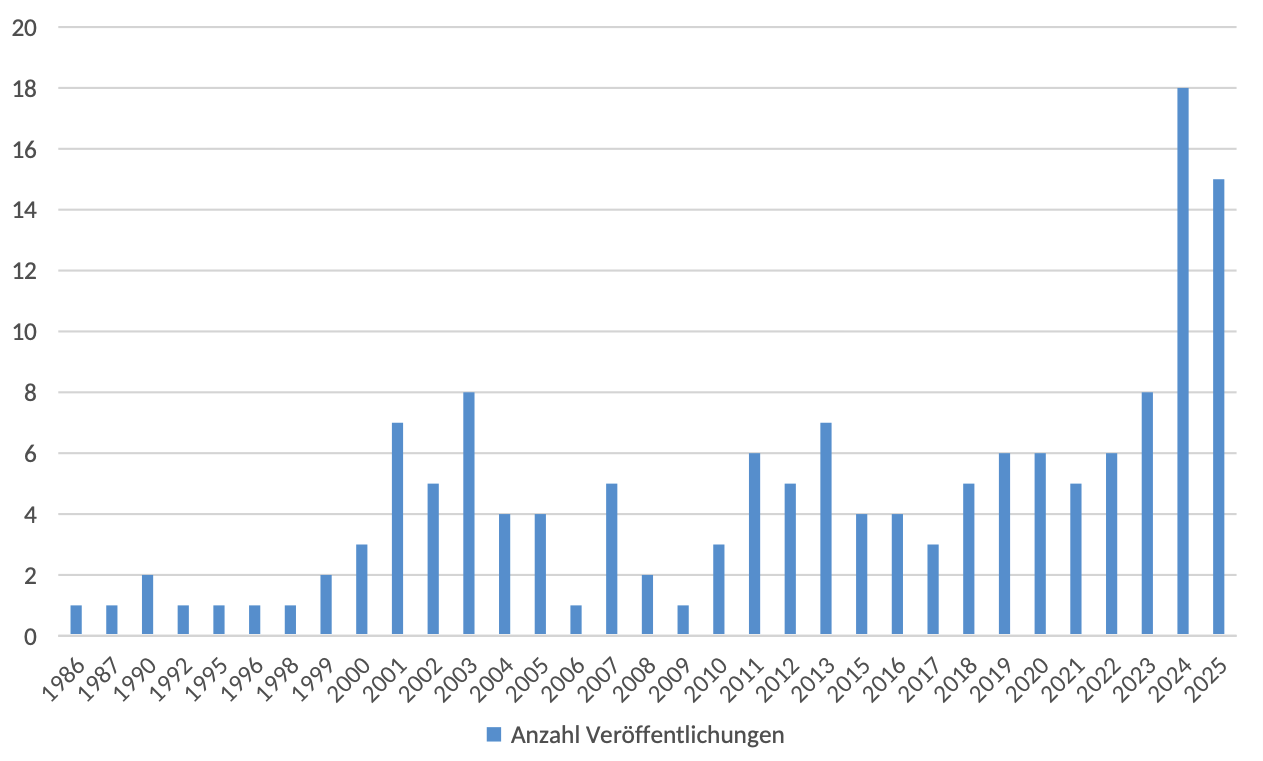
\includegraphics[width=0.90\textwidth]{graphics_lit/1-veroeffentlichungen-jahr.png}
    \caption{Übersicht der Veröffentlichungen pro Jahr}
    \label{fig:1-veroeffentlichungen-jahr}
\end{figure}

Aus Abbildung~\ref{fig:2-typ} ist ersichtlich, dass insgesamt 98~\% der Veröffentlichungen auf Journalartikel (ca. 36~\%) und Konferenzbeiträge (ca. 62~\%) entfallen. Während Journalartikel in Fachzeitschriften mit ausführlicherem Begutachtungsprozess erscheinen, werden Konferenzbeiträge überwiegend in Tagungsbänden veröffentlicht und dienen der schnellen Verbreitung aktueller Forschungsergebnisse \cite{abbadia_conference_2022}. Beide Publikationstypen sind daher für eine Trendanalyse sowie zur Ableitung von Best Practices geeignet.

\begin{figure}[!htbp]
    \centering
    % --- linke Seite: Grafik ---
    \begin{subfigure}[b]{0.48\textwidth}
        \centering
        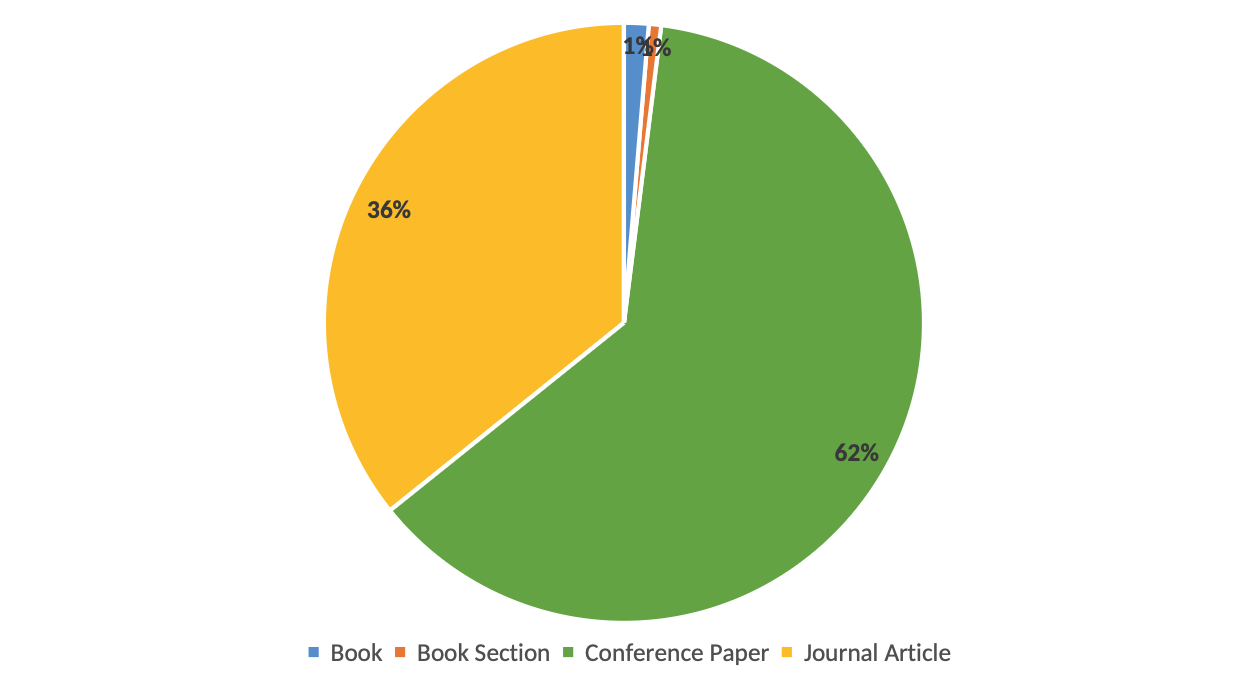
\includegraphics[width=1\textwidth]{graphics_lit/2-typ.png}
        \caption{Übersicht des Typs} 
        \label{fig:2-typ}
    \end{subfigure}
    \hfill
    % 
    % --- rechte Seite: Tabelle ---
    \begin{subfigure}[b]{0.48\textwidth}
        \centering
        \tiny
        \begin{tabularx}{\textwidth}{X c}
            \hline
            \multicolumn{2}{l}{\textbf{Journals}} \\
            \hline
            IEEE Transactions on Education & 10 \\
            Computer Applications in Engineering Education & 7 \\
            Journal on Educational Resources in Computing & 7 \\
            \hline
            \multicolumn{2}{l}{\textbf{Konferenzen}} \\
            \hline
            Workshop on Computer Architecture Education & 8 \\
            ACM Technical Symposium on Computer Science Education & 7 \\
            Annual International Symposium on Computer Architecture & 6 \\
            \hline
        \end{tabularx}
        \caption{Meistgenutzte Journals und Konferenzen}
        \label{tab:2-typ-detail}
    \end{subfigure}
    %
    \caption{Informationen zum Typ der Publikationen}
    \label{fig:2-typ-gesamt}
\end{figure}

Tabelle~\ref{tab:2-typ-detail} bietet eine Übersicht über die Zeitschriften und Konferenzen, in denen die meisten der untersuchten Publikationen veröffentlicht wurden. Die drei genannten Zeitschriften vereinen 44~\% aller Journalartikel, während die drei aufgeführten Konferenzen rund 22~\% der Konferenzbeiträge ausmachen.

Abbildung~\ref{fig:3-anzahl-themen} verdeutlicht, dass die häufigsten Themen der untersuchten Publikationen \enquote{Prozessoren und Architekturen} (44~\%), \enquote{Speicher und Performance} (11~\%) sowie \enquote{Hardware und Logistik} (10~\%) sind. Diese drei Themen umfassen zusammen rund 70~\% aller Publikationen. Dicht darauf folgen die Themen \enquote{Grundlagen und Theorien} sowie \enquote{Programmierung} mit jeweils 9~\% der Arbeiten.

\begin{figure}[!h]
    \centering
    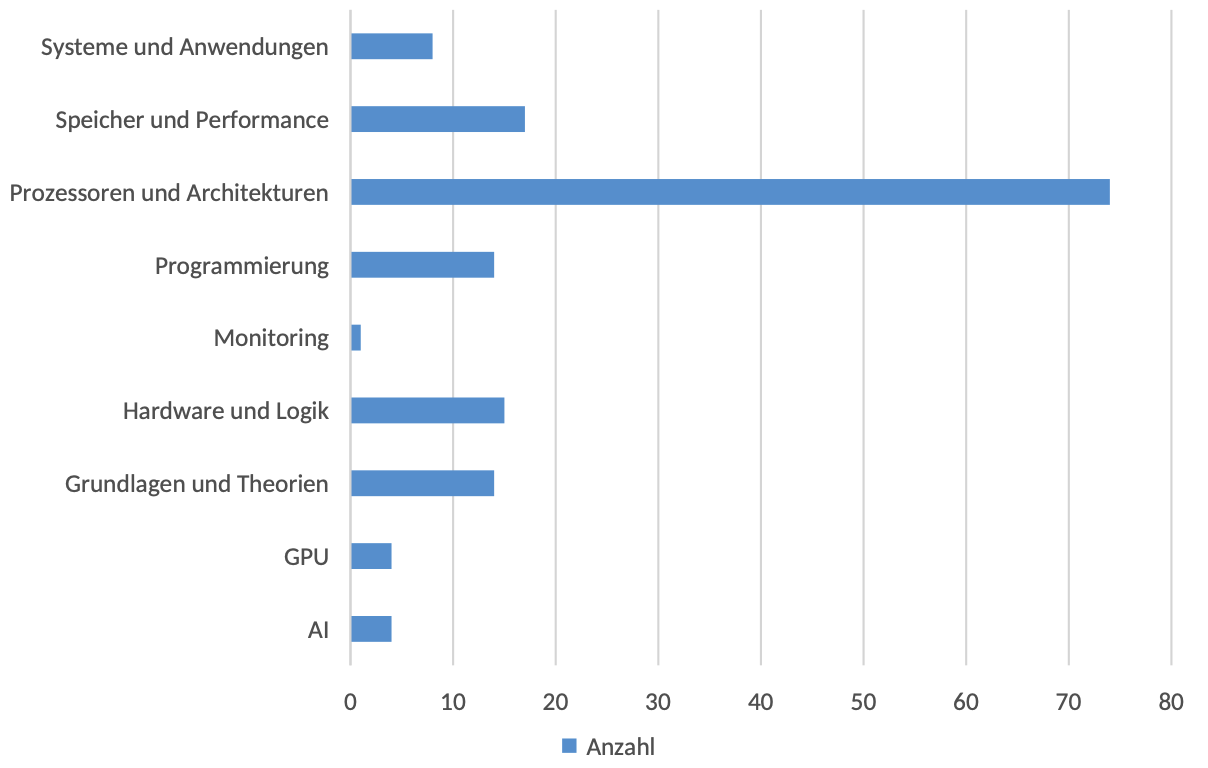
\includegraphics[width=0.90\textwidth]{graphics_lit/3-thema.png}
    \caption{Anzahl der Veröffentlichungen pro Thema}
    \label{fig:3-anzahl-themen}
\end{figure}

Eine detaillierte Untersuchung der drei am häufigsten vertretenen Themen ist in Abbildung~\ref{fig:4-top3-themen} dargestellt. Diese Grafik zeigt die Verteilung dieser Themen über verschiedene Zeitspannen. Die zugrunde liegenden Werte sind in der Tabelle~\ref{tab:themen-zeit} aufgeführt.

\begin{figure}[!htbp]
    \centering
    % --- linke Seite: Grafik ---
    \begin{subfigure}[b]{0.48\textwidth}
        \centering
        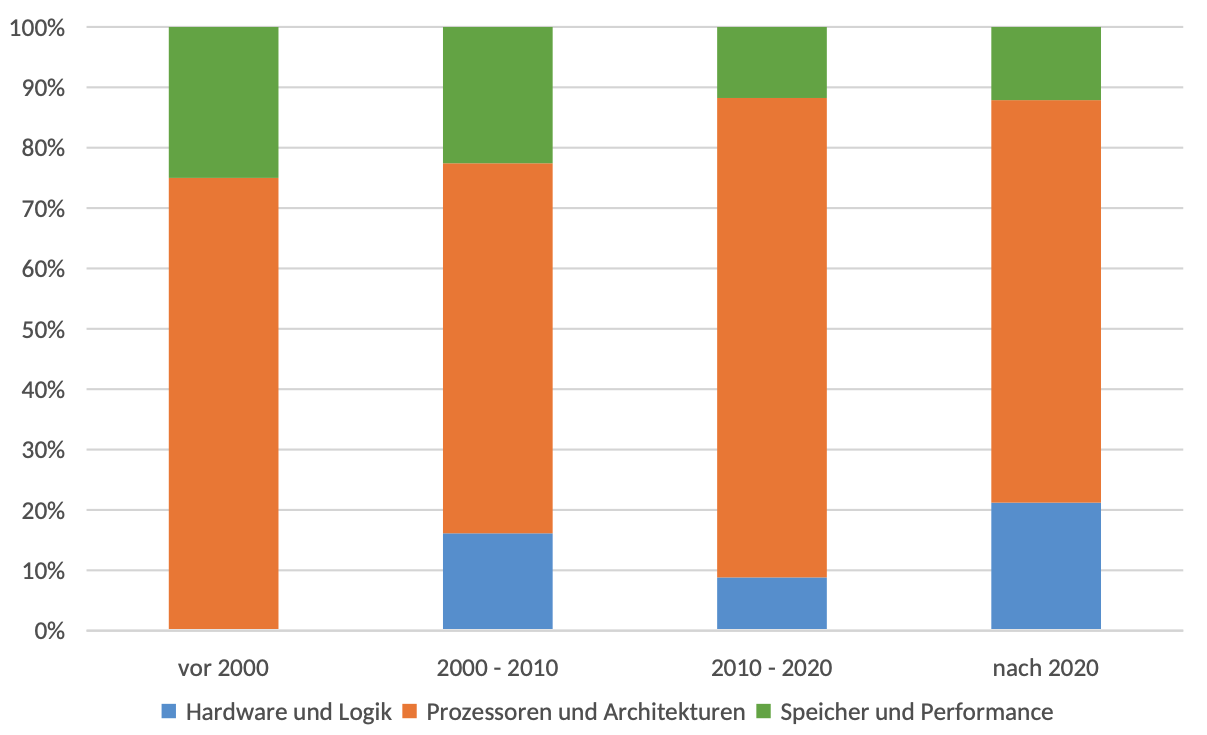
\includegraphics[width=0.90\textwidth]{graphics_lit/4-top3-themen-jahr.png}
        \caption{Jährliche Aufteilung Top 3 Themen (grafisch)}
        \label{fig:4-top3-themen}
    \end{subfigure}
    \hfill
    % 
    % --- rechte Seite: Tabelle ---
    \begin{subfigure}[b]{0.48\textwidth}
        \centering
        \tiny
        \begin{tabularx}{\textwidth}{lXXX}
            \hline
            \textbf{Zeitraum} & \textbf{Hardware und Logik} & \textbf{Prozessoren und Architekturen} & \textbf{Speicher und Performance} \\
            \hline
            vor 2000      & 0  & 6  & 2 \\
            2000--2010    & 5  & 19 & 7 \\
            2010--2020    & 3  & 27 & 4 \\
            nach 2020     & 7  & 22 & 4 \\
            \hline
        \end{tabularx}
        \caption{Jährliche Aufteilung Top 3 Themen (detailliert)}
        \label{tab:themen-zeit}
    \end{subfigure}
    %
    \caption{Jährliche Aufteilung Top 3 Themen}
    \label{fig:pub-typen}
\end{figure}

Für die Themen \enquote{Grundlagen und Theorien} sowie \enquote{Programmierung} zeigt Abb.~\ref{fig:5-top5-themen} die jährliche Verteilung. Die entsprechenden Werte sind in Tab.~\ref{tab:themen-zeit-2} aufgeführt. Auf eine detaillierte Analyse der verbleibenden Themen wir hier verzichtet. In dem Kapitel~\ref{chap:5-discussion} werde die Entwicklung aller Themen aufgegriffen und analysiert.

\begin{figure}[!htbp]
    \centering
    % --- linke Seite: Grafik ---
    \begin{subfigure}[b]{0.48\textwidth}
        \centering
        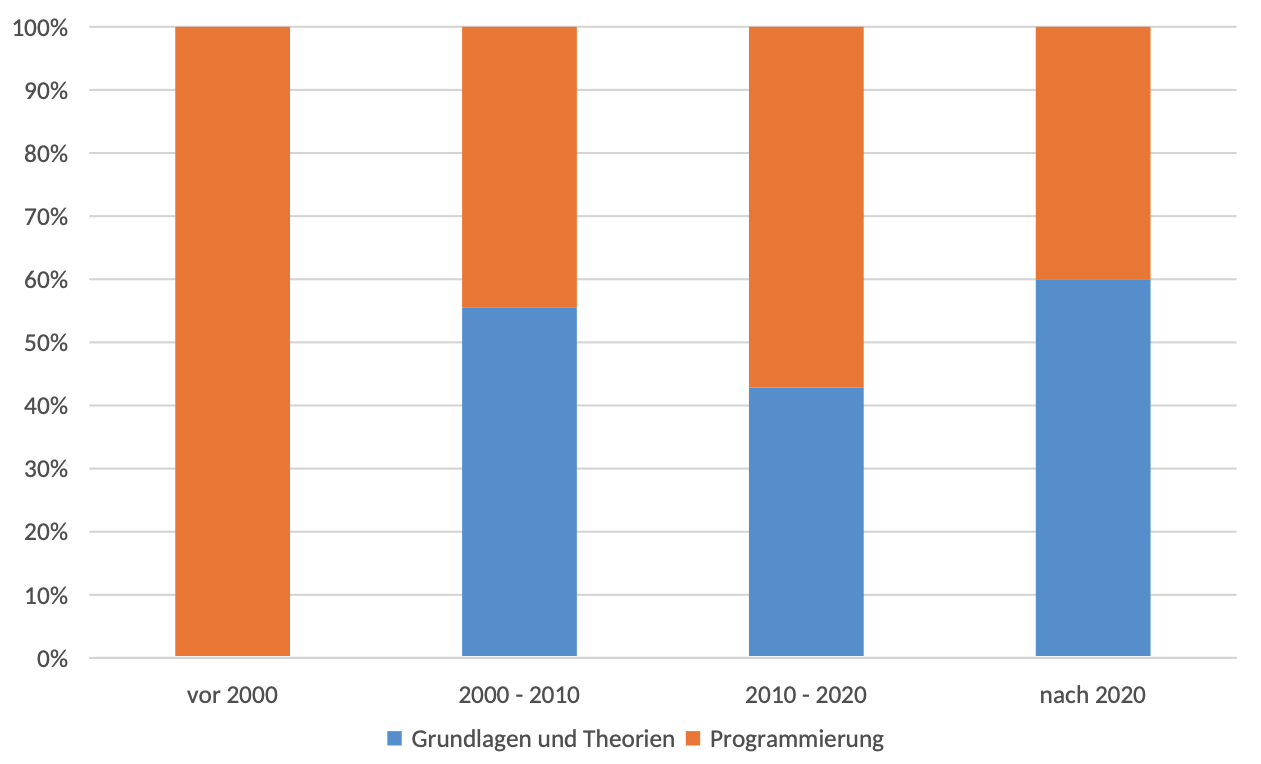
\includegraphics[width=0.90\textwidth]{graphics_lit/5-top5-themen-jahr.png}
        \caption{Jährliche Aufteilung weitere Themen (grafisch)}
        \label{fig:5-top5-themen}
    \end{subfigure}
    \hfill
    % 
    % --- rechte Seite: Tabelle ---
    \begin{subfigure}[b]{0.48\textwidth}
        \centering
        \tiny
        \begin{tabularx}{\textwidth}{lXX}
            \hline
            \textbf{Zeitraum} & \textbf{Grundlagen und Theorien} & \textbf{Programmierung} \\
            \hline
            vor 2000      & 0 & 2 \\
            2000--2010    & 5 & 4 \\
            2010--2020    & 3 & 4 \\
            nach 2020     & 6 & 4 \\
            \hline
        \end{tabularx}
        \caption{Jährliche Aufteilung weitere Themen (detailliert)}
        \label{tab:themen-zeit-2}
    \end{subfigure}
    %
    \caption{Jährliche Aufteilung weitere Themen}
    \label{fig:pub-typen}
\end{figure}

Hinsichtlich der Frage, ob die untersuchten Simulatoren spielerische Elemente (\textit{Gamification}) enthalten, bietet die Tabelle~\ref{tab:gamification} einen Überblick.

\begin{table}[!htbp]
    \centering
    \tiny
    \begin{tabular}{l c c}
        \hline
        \textbf{Gamification} & \textbf{Anzahl} & \textbf{\%} \\
        \hline
        Keine Elemente     & 145 & 96\% \\
        Elemente vorhanden & 6   & 4\%  \\
        \hline
        \textbf{Summe}     & 151 & 100\% \\
        \hline
    \end{tabular}
    \caption{Verteilung der Publikationen in Bezug auf enthaltene Gamification-Elemente}
    \label{tab:gamification}
\end{table}

Von den 151 Simulatoren der untersuchten wissenschaftlichen Publikationen wurden 15~\% als realitätsnah und 85~\% als didaktisch reduziert eingestuft. Die Verteilung bezogen auf die einzelnen Themenbereiche ist in Abbildung~\ref{fig:7-abstraktion-themen} dargestellt.

Die Abbildung~\ref{fig:8-abstraktion-jahr} verdeutlicht die zeitliche Entwicklung des Abstraktionslevels.

\begin{figure}[!htbp]
    \centering
    % --- linke Seite: Grafik ---
    \begin{subfigure}[b]{0.48\textwidth}
        \centering
        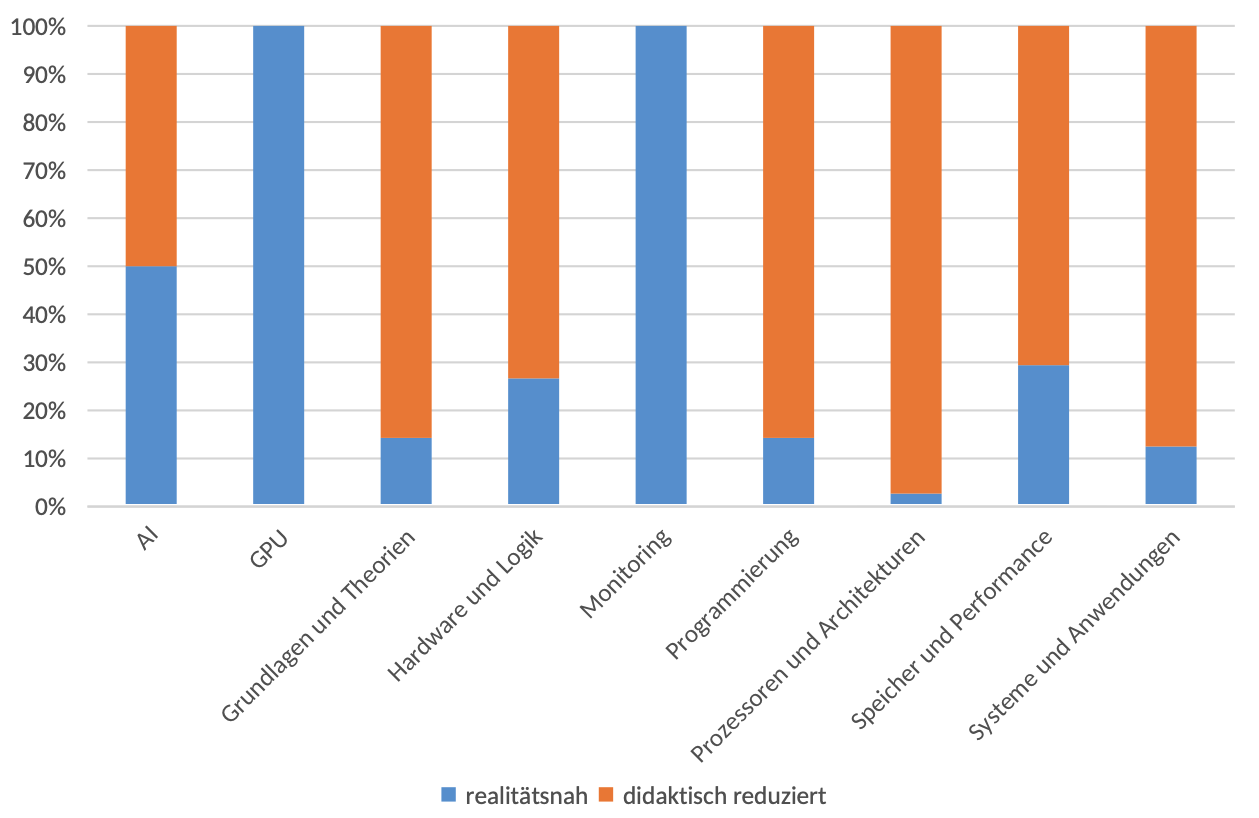
\includegraphics[width=0.90\textwidth]{graphics_lit/7-abtraktion-themen.png}
        \caption{Verteilung Abstraktionslevel auf Themen}
        \label{fig:7-abstraktion-themen}
    \end{subfigure}
    \hfill
    % 
    % --- rechte Seite: Grafik ---
    \begin{subfigure}[b]{0.48\textwidth}
        \centering
        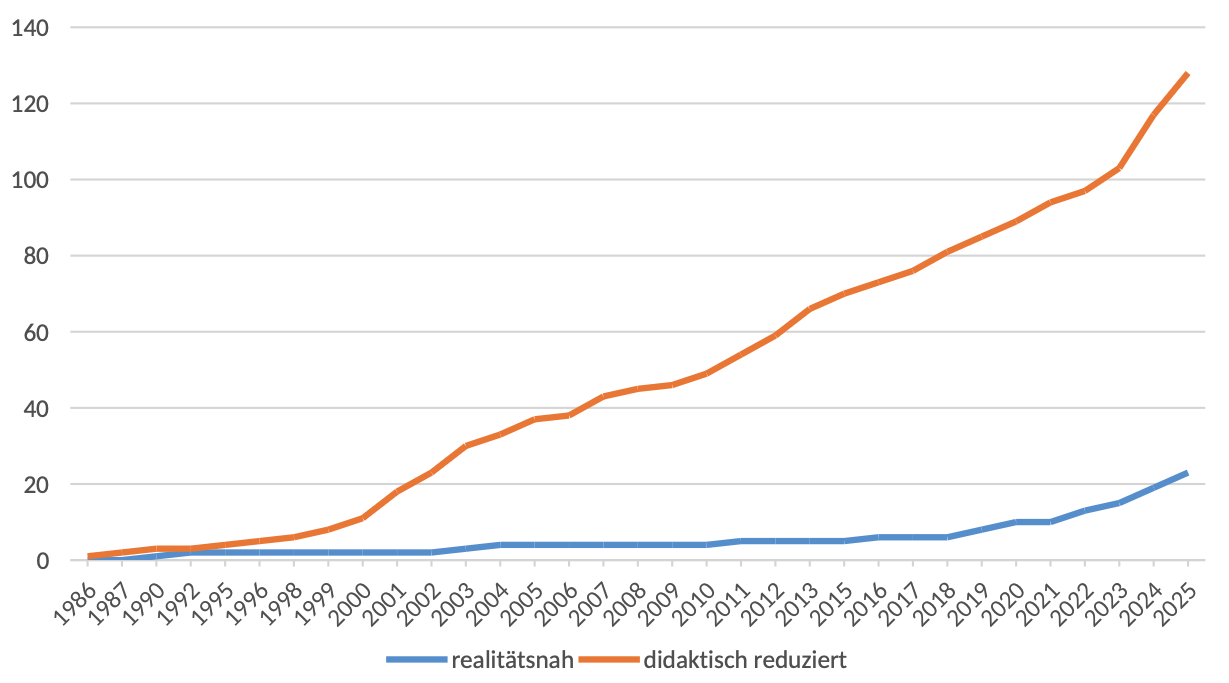
\includegraphics[width=0.90\textwidth]{graphics_lit/8-abstraktion-jahr.png}
        \caption{Zeitliche Entwicklung des Abstraktionslevels}
        \label{fig:8-abstraktion-jahr}
    \end{subfigure}
    %
    \caption{Analysen zum Abstraktionslevel}
    \label{fig:abstaktion-analysen}
\end{figure}

Anhand von Abbildung~\ref{fig:9-institution} ist zu erkennen, dass 89~\% der Publikationen die Hochschulbildung als Zielgruppe adressieren. 9~\% der untersuchten Simulatoren sind für Forschung und Beruf bestimmt, während sich die verbleibenden 2~\% auf schulische Bildung und Weiterbildungen aufteilen.

Untersucht man die Verteilung der Zielgruppen genauer, so zeigt Abbildung~\ref{fig:10-institution-themen} die Aufteilung der einzelnen Zielgruppen (\enquote{Schule}, \enquote{Hochschule}, \enquote{Forschung/Beruf}, \enquote{Weiterbildung}) auf die jeweiligen Themenbereiche. Dabei wird zum Beispiel deutlich, dass sich alle GPU-bezogenen Simulatoren der Forschungs- bzw. Berufsgruppe zuordnen lassen.

\begin{figure}[!htbp]
    \centering
    % --- linke Seite: Grafik ---
    \begin{subfigure}[b]{0.48\textwidth}
        \centering
        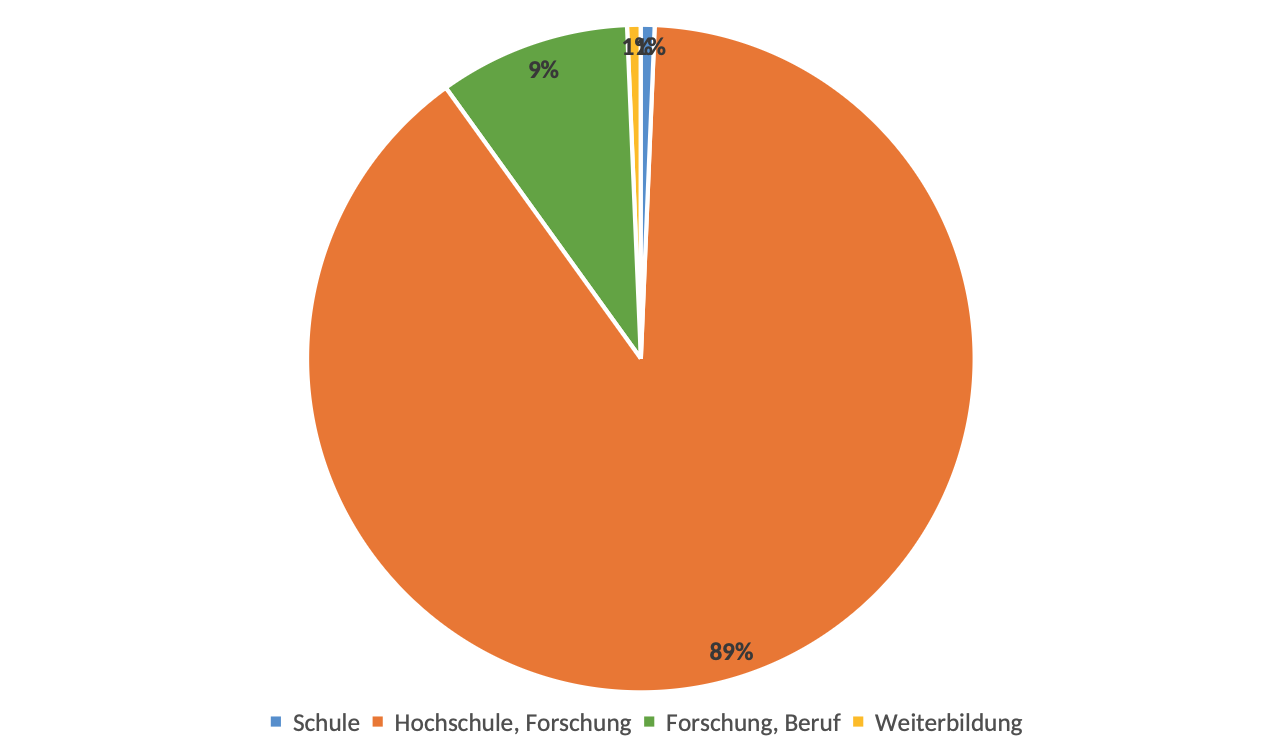
\includegraphics[width=0.90\textwidth]{graphics_lit/9-institution.png}
        \caption{Aufteilung Institutionen}
        \label{fig:9-institution}
    \end{subfigure}
    \hfill
    % 
    % --- rechte Seite: Grafik ---
    \begin{subfigure}[b]{0.48\textwidth}
        \centering
        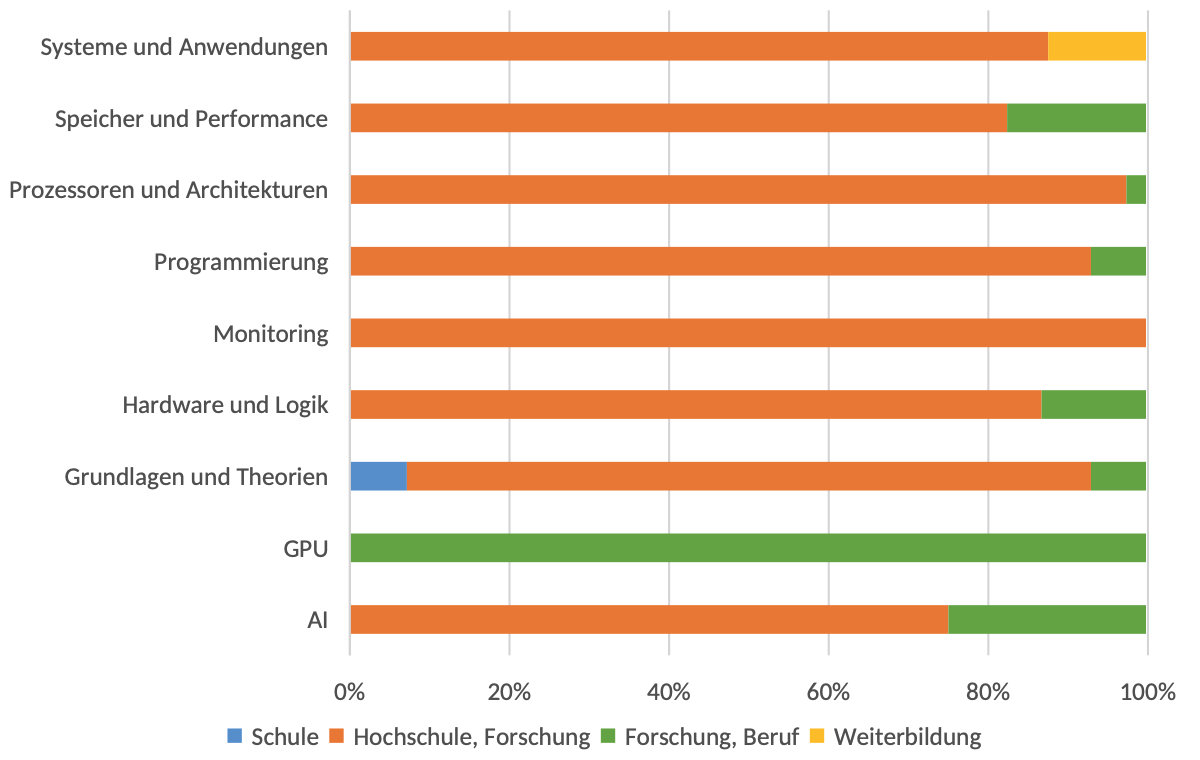
\includegraphics[width=0.90\textwidth]{graphics_lit/10-institution-themen.png}
        \caption{Aufteilung Institutionen nach Themen}
        \label{fig:10-institution-themen}
    \end{subfigure}
    %
    \caption{Analysen zu Institutionen}
    \label{fig:institution-analysen}
\end{figure}

Hinsichtlich des Zugriffs zeigt Abbildung~\ref{fig:11-zugriff} eine detaillierte Aufteilung. Die meisten Simulatoren (ca. 66~\%) sind offline nutzbar, während 11~\% entweder ausschließlich online oder sowohl online als auch offline verfügbar sind. In 19 Publikationen (ca. 13~\%) finden sich keine Angaben zur Art der Nutzung.

\begin{figure}[!htbp]
    \centering
    % --- linke Seite: Grafik ---
    \begin{subfigure}[b]{0.48\textwidth}
        \centering
        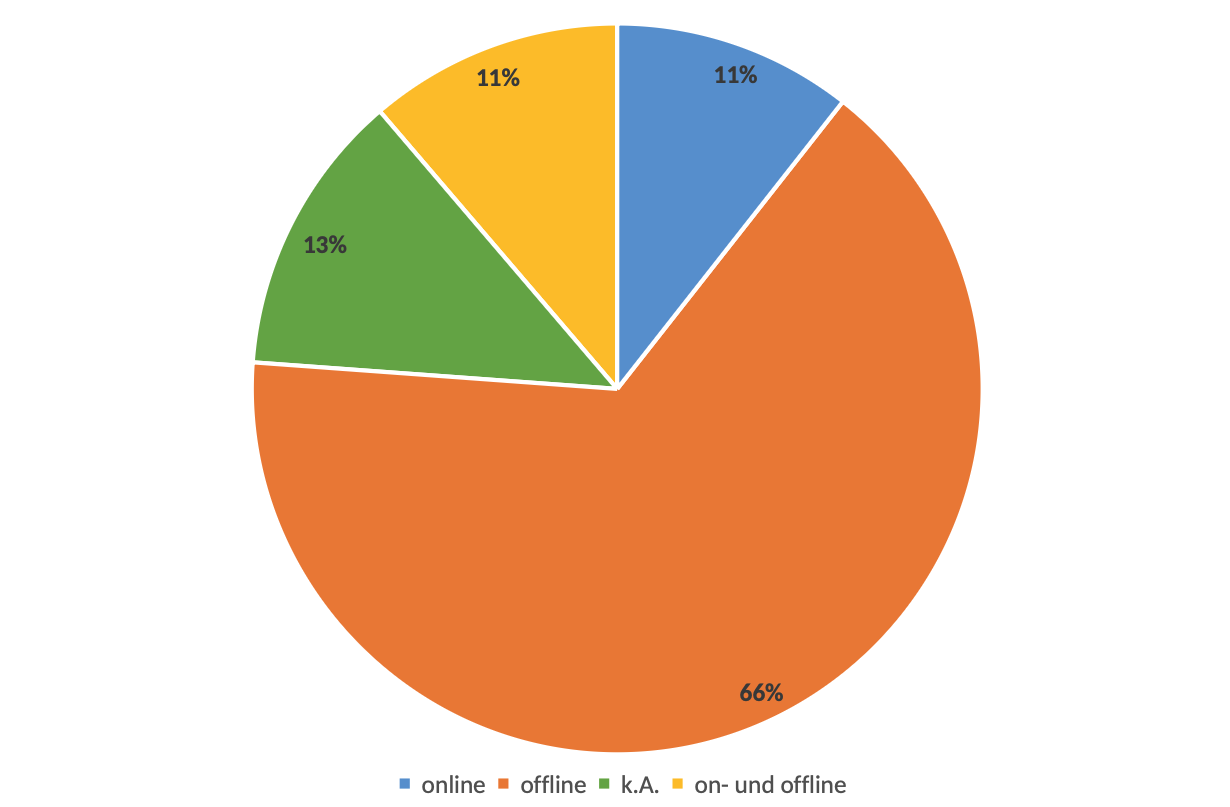
\includegraphics[width=0.90\textwidth]{graphics_lit/11-zugriff.png}
        \caption{Aufteilung Zugriff}
        \label{fig:11-zugriff}
    \end{subfigure}
    \hfill
    % 
    % --- rechte Seite: Grafik ---
    \begin{subfigure}[b]{0.48\textwidth}
        \centering
        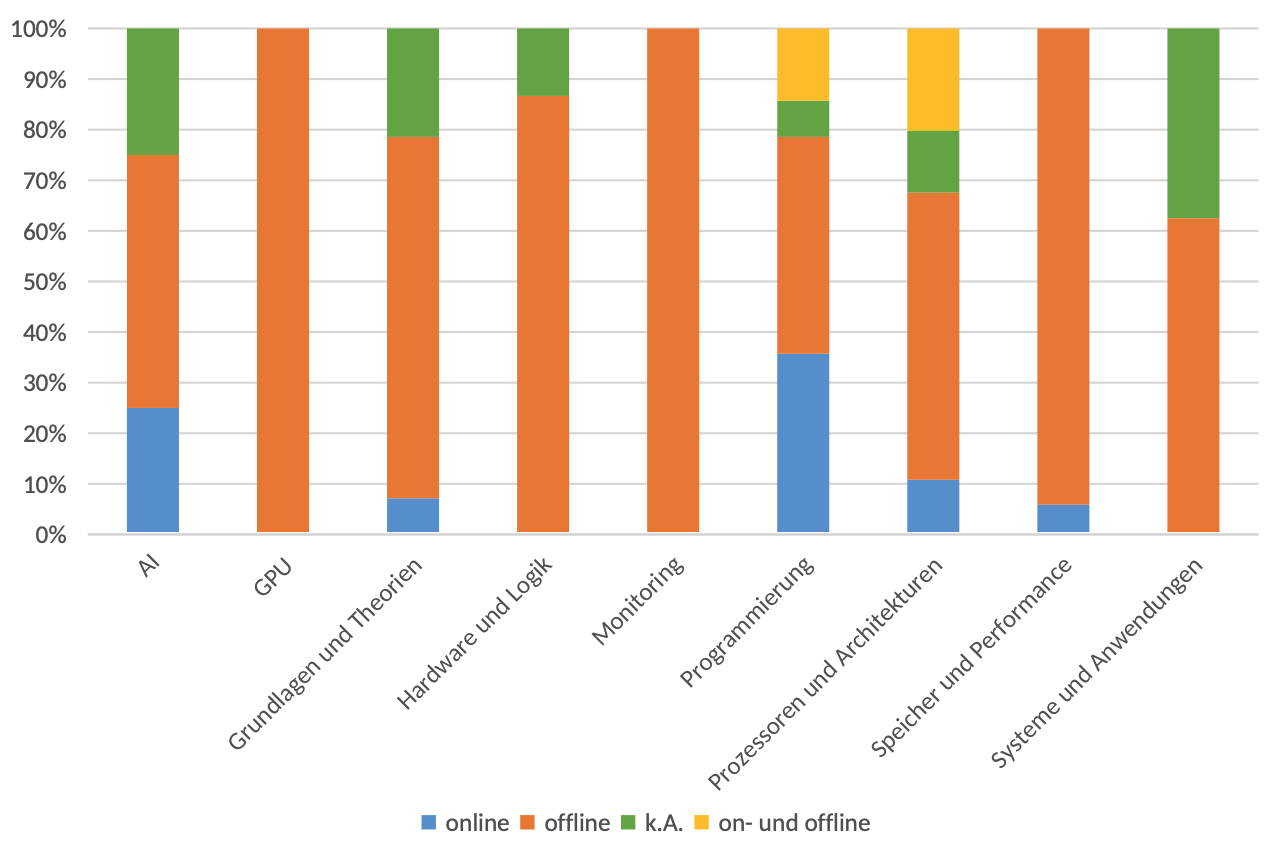
\includegraphics[width=0.90\textwidth]{graphics_lit/13-zugriff-thema.png}
        \caption{Zugriffsart pro Thema}
        \label{fig:13-zugriff-thema}
    \end{subfigure}
    %
    \caption{Analysen zu zum Zugriff}
    \label{fig:zugriff-analysen}
\end{figure}

Die zeitliche Verteilung der verschiedenen Zugriffsarten ist in Abbildung~\ref{fig:12-zugriff-jahr} dargestellt, die entsprechenden Werte sind in Tab.~\ref{tab:zugriff-zeit} aufgeführt.

\begin{figure}[!htbp]
    \centering
    % --- linke Seite: Grafik ---
    \begin{subfigure}[b]{0.48\textwidth}
        \centering
        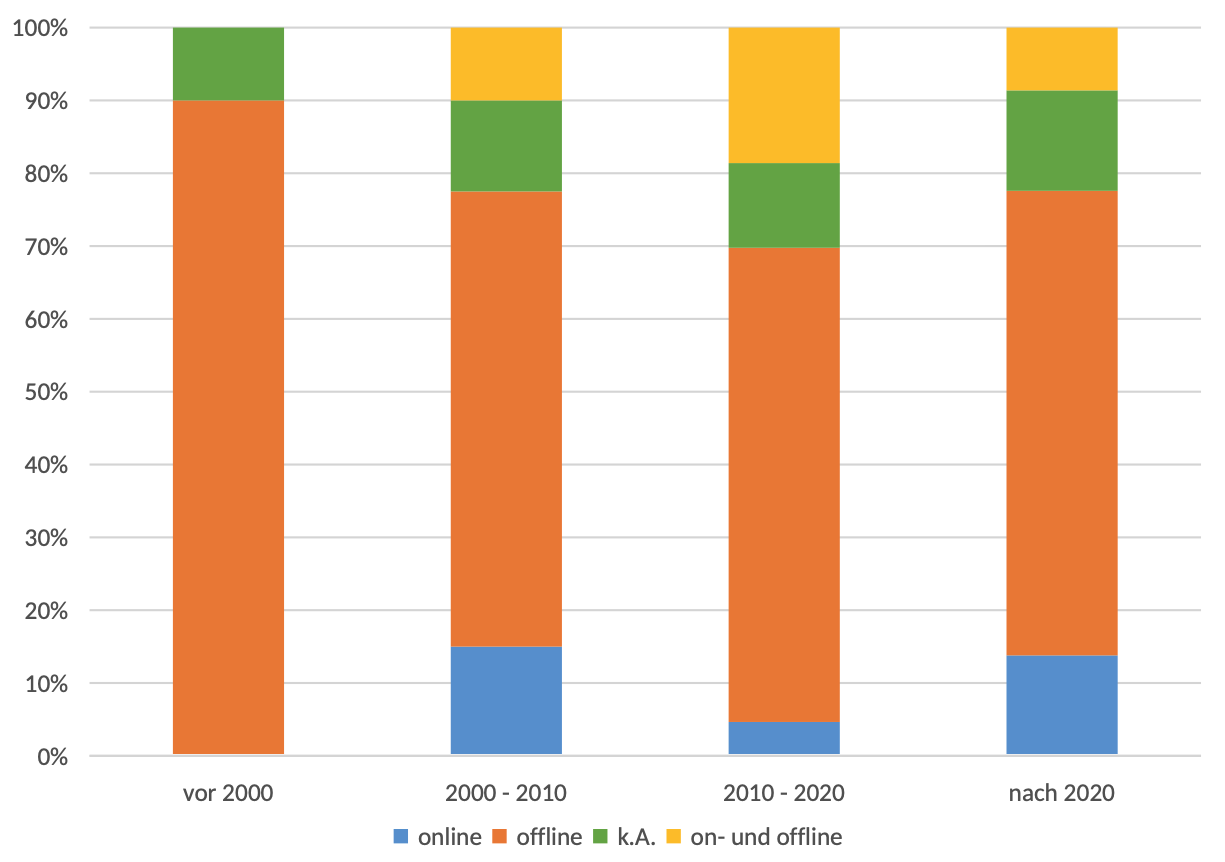
\includegraphics[width=\textwidth]{graphics_lit/12-zugriff-jahr.png}
        \caption{Jährliche Aufteilung Zugriff (grafisch)}
        \label{fig:12-zugriff-jahr}
    \end{subfigure}
    \hfill
    % 
    % --- rechte Seite: Tabelle ---
    \begin{subfigure}[b]{0.48\textwidth}
        \centering
        \tiny
        \begin{tabularx}{\textwidth}{lXXXX}
            \hline
            \textbf{Zeitraum} & \textbf{online} & \textbf{offline} & \textbf{keine Info} & \textbf{on-/offline} \\
            \hline
            vor 2000      & 0  & 9  & 1 & 0 \\
            2000--2010    & 6  & 25 & 5 & 4 \\
            2010--2020    & 2  & 28 & 5 & 8 \\
            nach 2020     & 8  & 37 & 8 & 5 \\
            \hline
        \end{tabularx}
        \caption{Jährliche Aufteilung Zugriff (detailliert)}
        \label{tab:zugriff-zeit}
    \end{subfigure}
    %
    \caption{Darstellung der Zugriffsarten pro Zeitraum}
    \label{fig:zugriff-gesamt}
\end{figure}

Abbildung~\ref{fig:13-zugriff-thema} zeigt die Verteilung der verschiedenen Zugriffsarten in Bezug auf die einzelnen Themenbereiche. Simulatoren, die auf Hardware wie \ac{FPGA}s basieren, werden der Kategorie \enquote{offline} zugeordnet.

Als zusätzliches Kriterium wurde der Preis untersucht, wobei zwischen \enquote{kostenlos} und \enquote{kostenpflichtig} unterschieden wird. Der Anteil der kostenlos verfügbaren didaktischen Simulatoren beträgt 57~\%, während 7~\% kostenpflichtig sind. Für die übrigen Simulatoren liegen keine Angaben zur preislichen Gestaltung vor (vgl. Abbildung~\ref{fig:14-preis2}). 

Darüber hinaus werden die Preiskategorien nach Zeiträumen aufgeschlüsselt, um einen Überblick über mögliche Veränderungen des Verhältnisses von kostenlosen zu kostenpflichtigen Simulatoren zu erhalten (vgl. Abbildung~\ref{fig:15-preis-gesamt}).

\begin{figure}[!htbp]
    \centering
    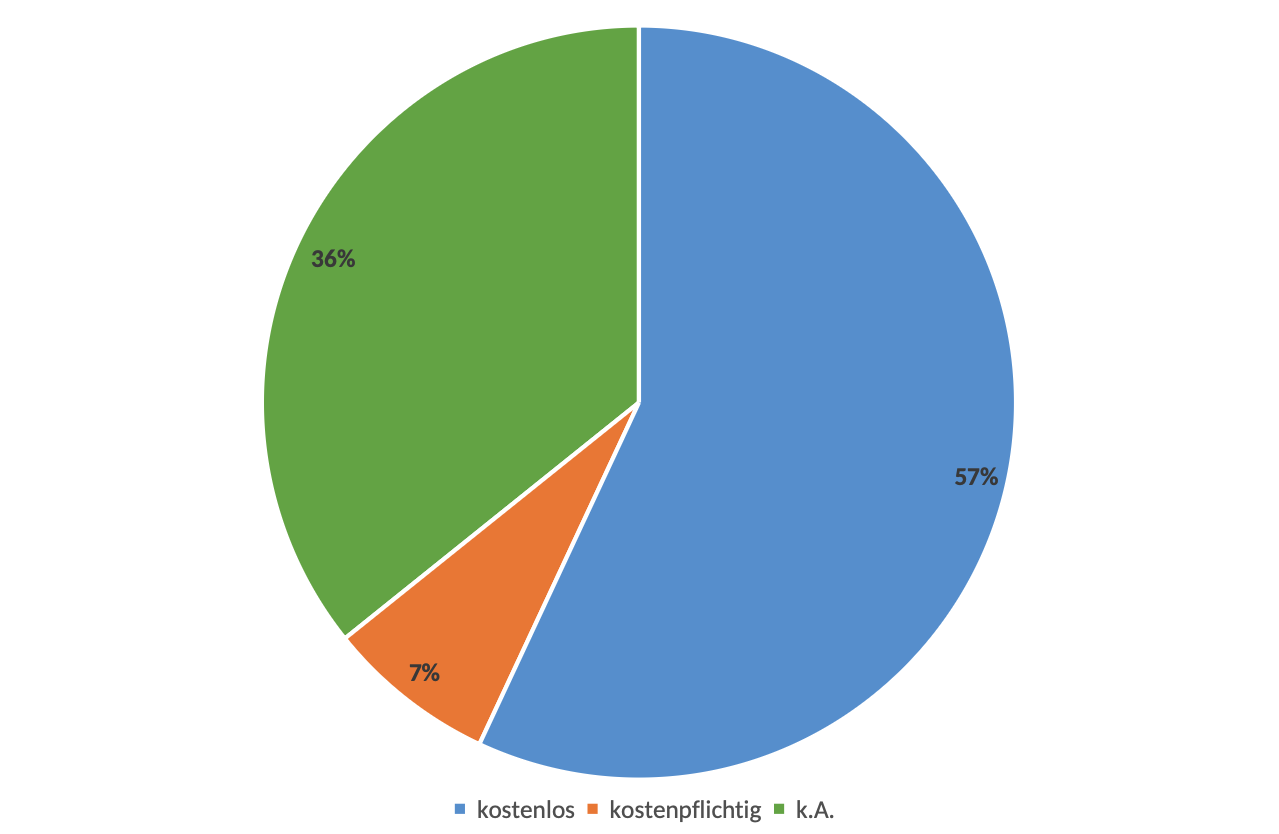
\includegraphics[width=0.9\textwidth]{graphics_lit/14-preis.png}
    \caption{Aufteilung Preis}
    \label{fig:14-preis2}
\end{figure}

\begin{figure}[!htbp]
    \centering
    % --- linke Seite: Grafik ---
    \begin{subfigure}[b]{0.48\textwidth}
        \centering
        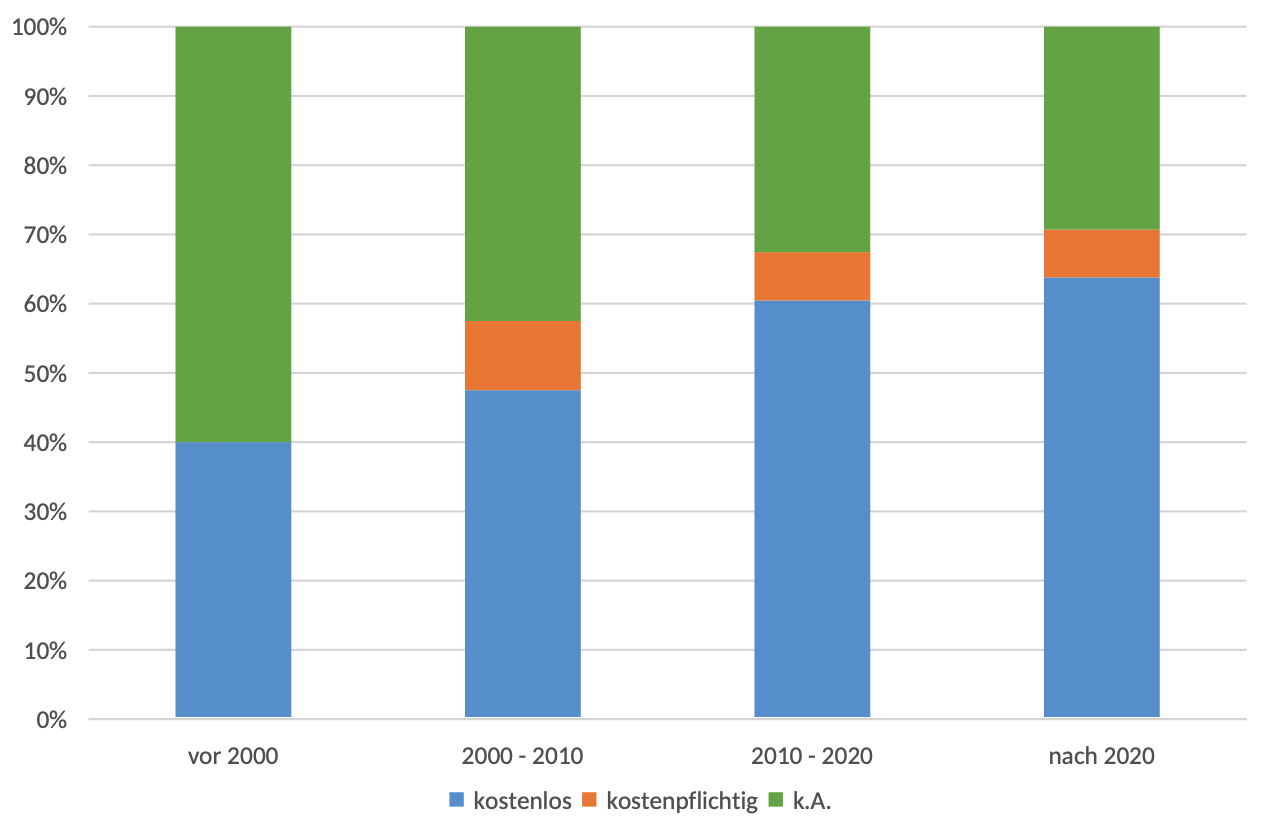
\includegraphics[width=\textwidth]{graphics_lit/15-preis-jahr.png}
        \caption{Aufteilung Preis (grafisch)}
        \label{fig:15-preis-jahr}
    \end{subfigure}
    \hfill
    % --- rechte Seite: Tabelle ---
    \begin{subfigure}[b]{0.48\textwidth}
        \centering
        \tiny
        \begin{tabularx}{\textwidth}{lXXX}
            \hline
            \textbf{Zeitraum} & \textbf{kostenlos} & \textbf{kostenpflichtig} & \textbf{k.A.} \\
            \hline
            vor 2000      & 4  & 0 & 6  \\
            2000--2010    & 19 & 4 & 17 \\
            2010--2020    & 26 & 3 & 14 \\
            nach 2020     & 37 & 4 & 17 \\
            \hline
        \end{tabularx}
        \caption{Aufteilung Preis (detailliert)}
        \label{tab:15-preis-zeit}
    \end{subfigure}
    %
    \caption{Darstellung der Preisgestaltung der Simulatoren über verschiedene Zeiträume}
    \label{fig:15-preis-gesamt}
\end{figure}

In Bezug auf das Kriterium \textit{Dokumentation} gibt Abbildung~\ref{fig:16-dokumentation} genauere Einblicke. In 87~\% der analysierten Publikationen verfügen die verwendeten bzw. beschriebenen Simulatoren über eine Dokumentation, während 5~\% keine Dokumentation erwähnen und in 7~\% der Publikationen hierzu keine Angaben vorliegen.

\begin{figure}[!htbp]
    \centering
    \caption{Aufteilung Dokumentation}
    \label{fig:16-dokumentation}
    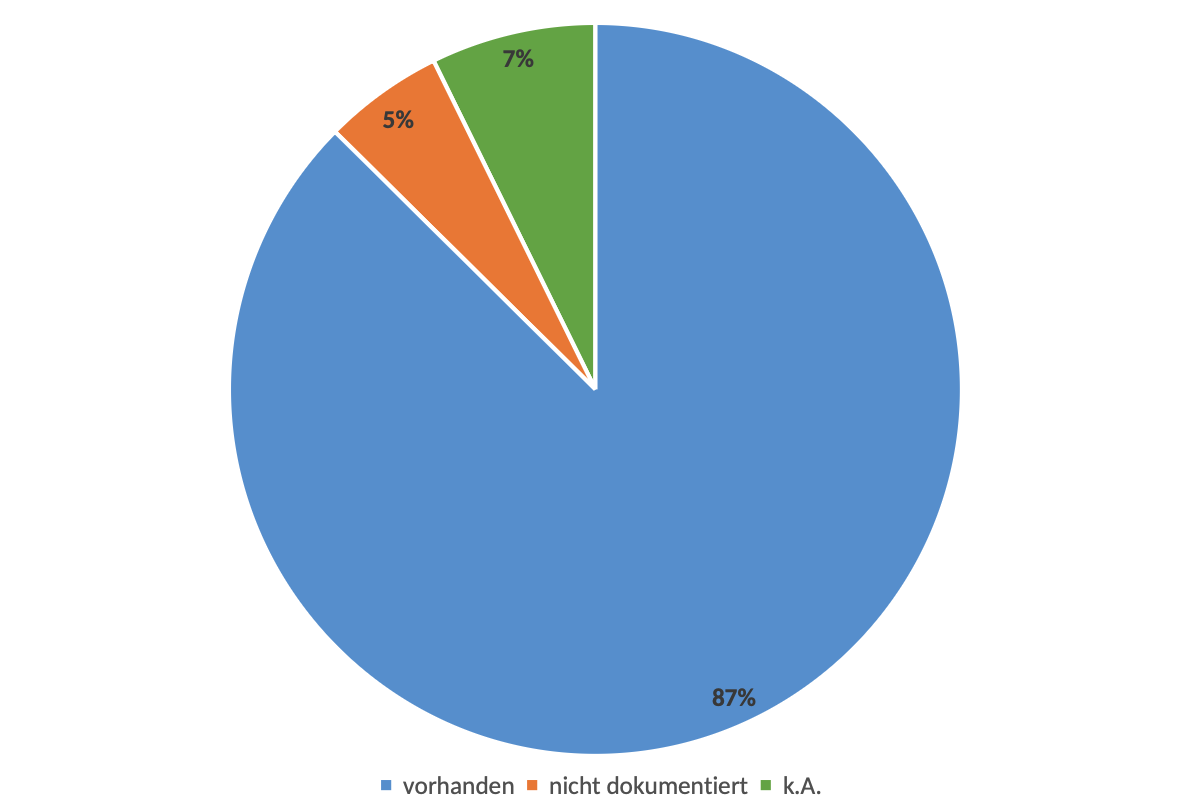
\includegraphics[width=0.90\textwidth]{graphics_lit/16-dokumentation.png}
\end{figure}

Als abschließendes Kriterium wird die Anzahl der Zitationen untersucht. Tabelle~\ref{tab:zitationen} zeigt die am häufigsten zitierten Publikationen pro Thema, da diese für weiterführende oder aufbauende Untersuchungen in den jeweiligen Bereichen als maßgeblich gelten. Die Auswahl der dargestellten Publikationen erfolgte auf Grundlage des Durchschnitts aller Zitationen, der bei etwa 35 liegt. Publikationen mit mehr als 35 Zitationen werden nachfolgend dargestellt.

{
\tiny
\centering
\begin{longtable}{|c|p{6cm}|p{3cm}|c|}
    \caption{Häufig zitierte Publikationen pro Themengebiet\label{tab:zitationen}} \\
    \hline
    \textbf{Zitationen} & \textbf{Titel} & \textbf{Autor(en)} & \textbf{Jahr} \\
    \hline
    \endfirsthead

    \hline
    \textbf{Zitationen} & \textbf{Titel} & \textbf{Autor(en)} & \textbf{Jahr} \\
    \hline
    \endhead

    \hline
    \multicolumn{4}{l}{Fortsetzung auf der nächsten Seite} \\
    \hline
    \endfoot

    \hline
    \endlastfoot

    % --- Inhalte ---
    \multicolumn{4}{c}{\textbf{AI}} \\
    \hline
    211 & Teaching CS50 with AI: Leveraging Generative Artificial Intelligence in Computer Science Education & R. Liu, C. Zenke, C. Liu, A. Holmes, P. Thornton, D. J. Malan & 2024 \\
    \hline
    \multicolumn{4}{c}{\textbf{GPU}} \\
    \hline
    146 & MGPUSim: Enabling Multi-GPU Performance Modeling and Optimization & Y. Sun, T. Baruah, S. A. Mojumber, S. Dong, X. Gong, S. Treadway & 2019 \\
    397 & Accel-Sim: An Extensible Simulation Framework for Validated GPU Modeling & M. Khairy, Z. Shen, T. M. Aamodt, T. G. Rogers & 2020 \\
    \hline
    \multicolumn{4}{c}{\textbf{Grundlagen und Theorien}} \\
    \hline
    117 & Flexible Web-Based Educational System for Teaching Computer Architecture and Organization & J. Djordjevic, B. Nikolic, A. Milenkovic & 2005 \\
    \hline
    \multicolumn{4}{c}{\textbf{Hardware und Logik}} \\
    \hline
    46 & Harnessing FPGAs for Computer Architecture Education & M. Holland, J. Harris, S. Hauck & 2003 \\
    \hline
    \multicolumn{4}{c}{\textbf{Programmierung}} \\
    \hline
    41 & Using Simulators for Teaching Computer Organization and Architecture & P. W. C. Prasad, A. Alsadoon, A. Beg, A. Chan & 2016 \\
    51 & MarieSim: The MARIE Computer Simulator & L. Null, J. Lobur & 2003 \\
    \hline
    \multicolumn{4}{c}{\textbf{Prozessoren und Architekturen}} \\
    \hline
    162 & Control Flow Modeling in Statistical Simulation for Accurate and Efficient Processor Design Studies & L. Eeckhout, R. H. Bell, B. Stougie, K. De Bosschere, L. K. John & 2004 \\
    172 & Applying a Constructivist and Collaborative Methodological Approach in Engineering Education & L. Moreno, C. Gonzalez, I. Castilla, E. Gonzalez, J. Sigue & 2007 \\
    327 & Measuring Experimental Error in Microprocessor Simulation & R. Desikan, D. Burger, S. W. Keckler & 2001 \\
    \hline
    \multicolumn{4}{c}{\textbf{Speicher und Performance}} \\
    \hline
    53 & Cryogenic Computer Architecture Modeling with Memory-Side Case Studies & L. Gyu-Hyeon, M. Dongmoon, B. Ilkwon, K. Jangwoo & 2019 \\
    205 & A Simulation Based Study of TLB Performance & A. Borg, J. B. Chen, N. P. Jouppi & 1992 \\
    \hline
    \multicolumn{4}{c}{\textbf{Systeme und Anwendungen}} \\
    \hline
    139 & Virtual Reality in Computer Science Education: A Systematic Review & J. Priker, A. Dengel, M. Holly, S. Safikani & 2020 \\
    \hline
\end{longtable}
}





\section{Ergebnisse aus Tabelle~\ref{tab:simulatoren}}

test test


\chapter{Diskussion und Best Practices}\label{chap:5-discussion}

% E-Learning
E-Learning ist nicht das gelbe vom Ei\label{elearning}. Niegemann arbeitet in seinem Lehrbuch auf dem Jahr 2009 heraus, dass die Euphorie für E-Learning etwas seit 2002 abzuflachen schien, da viele Erwartungen nicht erfüllt würden.\parencite[S.~14]{niegemann_kompendium_2008}

\begin{itemize}
	\item Kosteneinsparungen könnten häufig nicht erzielt werden, sodass didaktisch wertvolle Lernsoftware mit erhöhten finanziellen Aufwendugen verbunden sei.
	\item Ob Texte und Bilder nun in einer Lernsoftware oder in einem Vorlesungsskript dargestellt werde, weise keinen großen Unterschied auf, da es lediglich Texte und Bilder blieben.
	\item Eine erhöhte Abbrruchrate beim E-Learning sei zu verzeichnen, da die Lernenden das selbstständige Lernen nicht gewohnt seien und keine hinreichende tutorielle Unterstützung erhielten.
	\item Der Zeitaufwand sei beim problembasierten bzw. entdeckenden Lernen in multimedialen Lernumgebungen hoch, sodass auch bei nachgewiesener Effektivität dieser Medien nicht alle Lerninhalte vermittelt werden könnten; die Effektivität des problembasierten Lernens sei zudem keineswegs belegt.
	\item In virtuellen Arbeitsgruppen im Web zeigten sich genau die gleichen Probleme, die von Präsenzarbeitsgruppen bekannt seien.
\end{itemize}

Trotz der oben genannten Schwierigkeiten verdeutlicht Niegemann, dass sich E-Learning als Lehr- und Lernform etabliert habe. Quelle der Probleme sei hier die mangelnde didaktische Konzeption dieser Programme.\parencite[S.~14]{niegemann_kompendium_2008}

% Mobile Learning
Gleichzeitig stellt Mobile Learning neue Anforderungen an Didaktik, Usability und Gestaltung von Lerninhalten, da Bildschirmgröße, Nutzungskontext und Interaktionsmöglichkeiten stärker variieren als bei Desktop-Systemen.

% Microlearning
Es lässt sich festhalten, dass Microlearning eine Reihe zentraler Vorteile bietet: Es fördert zum einen die Behaltensleistung durch die kompakte und wiederholbare Aufbereitung von Lerninhalten. Zum anderen steigert es die Lernendenmotivation und das Engagement, da Inhalte flexibel, kontextbezogen und in kurzen Einheiten vermittelt werden. Darüber hinaus unterstützt Microlearning auch kollaborative Lernprozesse in sozialen oder mobilen Umgebungen. Schließlich zeigen Studien, dass Microlearning die Lernfähigkeit und Leistung der Teilnehmenden insgesamt verbessern kann.\parencite[S.~2]{leong_review_2021}


\section{Trends und Herausforderungen}

\section{Empfehlungen für die Zukunft}

\chapter{Fazit}

Ziel dieser Arbeit war es, den Stand didaktischer Simulatoren für die Lehre der Rechnerarchitektur systematisch zu erfassen, vergleichbar zu machen und daraus Best Practices sowie Entwicklungsperspektiven abzuleiten. Durch die Analyse von 151 Publikationen und 57 veröffentlichten Simulatoren konnten zentrale thematische und didaktische Muster identifiziert werden.

Die Ergebnisse verdeutlichen klare Schwerpunkte: Prozessoren und Architekturen, insbesondere \acs{RISC}, bilden nach wie vor den Kernbereich der didaktischen Simulatoren. Zugleich gewinnen GPU-, KI-bezogene und immersive Ansätze zunehmend an Bedeutung und spiegeln die aktuellen technologischen Entwicklungen der Rechnerarchitektur wider. Damit lassen sich sowohl eine starke Kontinuität klassischer Inhalte als auch erste Verschiebungen hin zu neuen Themenfeldern beobachten.

Didaktisch wirksam sind vor allem reduzierte Darstellungen im Sinne der \acl{CTML}, da sie komplexe Sachverhalte auf wesentliche Kernelemente verdichten. Gamification wird bislang nur vereinzelt integriert, obwohl die Literatur deutliche Potenziale zur Steigerung der Lernmotivation belegt. Häufig genannte Erfolgsfaktoren sind darüber hinaus eine ortsunabhängige Nutzung (online oder hybrid), die Kostenfreiheit, plattformübergreifende Verfügbarkeit sowie eine umfassende und verlässliche Dokumentation. Zusammengenommen führen diese Befunde zu Empfehlungen für die zukünftige Gestaltung, Bereitstellung und didaktische Nutzung von Simulatoren.

Aus der Diskussion ergeben sich zwei zentrale Schlussfolgerungen: Erstens sollten Simulatoren gezielt für kleine, klar strukturierte Lerneinheiten konzipiert werden, die den Lernprozess schrittweise begleiten und bei Bedarf durch spielerische Elemente ergänzt werden können. Zweitens besteht eine deutliche Forschungslücke in Bezug auf belastbare empirische Studien, die den Einsatz dieser Werkzeuge in realen Lehrkontexten untersuchen. Zukünftige Arbeiten sollten daher (1) genauere und weniger subjektive Maße zur Einschätzung der Relevanz nutzen, (2) die Nutzungsdauer und Interaktionsmuster als Indikatoren für Qualität und Motivation erfassen und (3) den schulischen Bildungsbereich stärker berücksichtigen, da Simulatoren bislang vorwiegend in der Hochschullehre verankert sind.

Darauf aufbauend ergibt sich eine Forschungsagenda, die von methodisch fundierten Feldstudien bis hin zur Entwicklung klarer Kategorien reicht, mit denen sich die Unterschiede zwischen \enquote{Gamified Learning} und \enquote{Game-Based Learning} systematisch erfassen lassen. Für die Praxis bedeutet dies, dass Lehrende bereits heute auf eine Reihe Gestaltungsprinzipien zurückgreifen können, während die Forschung in den kommenden Jahren verstärkt Evidenz für Wirksamkeit und Transferfähigkeit liefern sollte. Auf diese Weise trägt die Arbeit sowohl zur theoretischen Fundierung als auch zur praktischen Weiterentwicklung didaktischer Simulatoren im Bereich der Rechnerarchitektur bei.



\cleardoublepage
\clearpage

\listoffigures
\clearpage

\listoftables
\clearpage

\appendix
\chapter{Relevante Tabellen}

\begin{landscape}
\fancyhf{} 
\renewcommand{\headrulewidth}{0pt} 
\fancyfoot[C]{\thepage} 
\tiny
\newcolumntype{L}[1]{>{\RaggedRight\arraybackslash}p{#1}}

% https://tableconvert.com/csv-to-latex
\begin{longtable}{|c|L{2cm}|p{2cm}|c|c|L{1.75cm}|L{1.5cm}|L{1.25cm}|c|c|c|c|c|c|c|}
    \caption{Ergebnisse Literaturrecherche} \label{tab:literatur} \\
    \hline
    \textbf{ID} & \textbf{Autor:innen} & \textbf{Titel} & \textbf{Jahr} & \textbf{Typ} & \textbf{Zeitschrift} & \textbf{Thema} & \textbf{Cluster} & \textbf{Gamification} & \textbf{Abstraktion} & \textbf{Institution} & \textbf{Zugriff} & \textbf{Preis} & \textbf{Dokumentation} & \textbf{Zitationen} \\ 
    \hline
    \hline
    \endfirsthead

    % Kopf auf den Folgeseiten
    \hline
    \textbf{ID} & \textbf{Autor:innen} & \textbf{Titel} & \textbf{Jahr} & \textbf{Typ} & \textbf{Zeitschrift} & \textbf{Thema} & \textbf{Cluster} & \textbf{Gamification} & \textbf{Abstraktion} & \textbf{Institution} & \textbf{Zugriff} & \textbf{Preis} & \textbf{Dokumentation} & \textbf{Zitationen} \\  
    \hline
    \hline
    \endhead

    % Fortsezung
    \hline
    \multicolumn{15}{l}{Fortsetzung nächste Seite} \\
    \hline
    \endfoot

    \hline
    \multicolumn{15}{l}{Ende der Tabelle} \\
    \hline
    \endlastfoot

    1 & P. W. C. Prasad, A. Alsadoon, A. Beg, A. Chan  & Using Simulators for Teaching Computer Organization And Architecture & 2016 & Journal Article & Computer Applications in Engineering Education & Assembler & Programmierung & 0 & 1 & 1 & 3 & 0 & 0 & 41 \\ \hline
    2 & Z. Radivojevic, Z. Stanisavljevic, M. Punt & Configurable Simulator For Computer Architecture And Organization & 2018 & Journal Article & Computer Applications in Engineering Education & Prozessor & Prozessoren und Architekturen & 0 & 1 & 1 & 2 & 2 & 2 & 9 \\ \hline
    3 & D. Camarmas-Alonso,  F. Garcia-Carballeira,  A. Calderon-Mateos,  E. del-Pozo-Punal & CREATOR: An Educational Integrated Development Environment for RISC-V Programming & 2024 & Journal Article & IEEE Access & RISC & Prozessoren und Architekturen & 0 & 1 & 1 & 0 & 0 & 0 & 4 \\ \hline
    4 & M. Dogan, K. Ötzoprak, M. Resit Tolun & Teaching Computer Architecture by Designing and Simulating Processors from their Bits and Bytes & 2024 & Journal Article & PeerJ Computer Science & MIPS & Prozessoren und Architekturen & 0 & 1 & 1 & 1 & 0 & 0 & 2 \\ \hline
    5 & P. Fuentes, C. Camarero, D. Herreros, V. Mateev, F. Vallejo, C. Martinez & Addressing Student Fatigue in Computer Architecture Courses & 2022 & Journal Article & IEEE Transactions on Learning Technologies & Einsatz echter Hardware & Hardware und Logik & 0 & 0 & 1 & 1 & 2 & 0 & 5 \\ \hline
    6 & L. Moreno, C. Gonzalez, I. Castilla, E. Gonzalez, J. Sigue & Applying a Constructivist and Collaborative Methodological Approach in Engineering Education & 2007 & Journal Article & Computers and Education & Superskalarität & Prozessoren und Architekturen & 0 & 1 & 1 & 3 & 0 & 0 & 172 \\ \hline
    7 & B. Garcia Fernandez, X. Del Toro, M. J. Santofimia, J. Dorado, F. J. Villanueva, D. Villa & Robotics vs. Game-Console-Based Platforms to Learn Computer Architecture & 2020 & Journal Article & IEEE Access & Einsatz echter Hardware & Hardware und Logik & 0 & 0 & 1 & 2 & 1 & 2 & 9 \\ \hline
    8 & D. Patti, A. Spadaccini, M. Palesi, F. Fazzino, V. Catania & Supporting Undergraduate Computer Architecture Students Using a Visual MIPS64 CPU Simulator & 2012 & Journal Article & IEEE Transactions on Education & MIPS & Prozessoren und Architekturen & 0 & 1 & 1 & 3 & 0 & 0 & 39 \\ \hline
    9 & J. Michelic, T Dobravec & SicSim: A Simulator of the Educational SIC/XE Computer for a System Software Course & 2015 & Journal Article & Computer Applications in Engineering Education & Prozessor & Prozessoren und Architekturen & 0 & 1 & 1 & 0 & 0 & 0 & 17 \\ \hline
    10 & J. H. Lee, S. S. Lee, H. Chang Yu, T. Su & Pipelined CPU Design With FPGA in Teaching Computer Architecture & 2012 & Journal Article & IEEE Transactions on Education & Pipelining & Prozessoren und Architekturen & 0 & 1 & 1 & 0 & 1 & 0 & 56 \\ \hline
    11 & S. Z. Sweidan, K. A. Darabkh & A new Efficient Assembly Language Teaching Aid for Intel Processors & 2015 & Journal Article & Computer Applications in Engineering Education & Assembler & Programmierung & 0 & 1 & 1 & 2 & 2 & 1 & 18 \\ \hline
    12 & L. Ribas-Xirgo & Yet Another Simple Processor (YASP) for Introductory Courses on Computer Architecture & 2010 & Journal Article & IEEE Transactions on Industrial Electronics & Prozessor & Prozessoren und Architekturen & 0 & 1 & 1 & 3 & 0 & 0 & 11 \\ \hline
    13 & J. Djordjevic, B. Nikolic, A. Milenkovic & Flexible Web-Based Educational System form Teaching Computer Architecture and Organization & 2005 & Journal Article & IEEE Transactions on Education & Rechnerarchitektur & Grundlagen und Theorien & 0 & 1 & 1 & 0 & 0 & 0 & 117 \\ \hline
    14 & S. N. Soares, F. R. Wagner & T$\backslash$\&D-Bench-Innovative Combined Support for Education and Research in Computer Architecture and Embedded Systems & 2011 & Journal Article & IEEE Transactions on Education & ADL & Grundlagen und Theorien & 0 & 1 & 1 & 2 & 2 & 2 & 15 \\ \hline
    15 & C. Gomez, M. E. Gomez, J. Sahuquillo & Bringing Real Processors to Labs & 2015 & Journal Article & Computer Applications in Engineering Education & Prozessor & Prozessoren und Architekturen & 0 & 1 & 1 & 1 & 0 & 0 & 4 \\ \hline
    16 & L. Moreno, E. J. Gonzales, B. Popescu, J. Toledo, J. Torres, C. Gonzales & MNEME: A Memory Hierarchy Simulator for an Engineering Computer Architecture Course & 2011 & Journal Article & Computer Applications in Engineering Education & Speicherhierarchie & Speicher und Performance & 0 & 1 & 1 & 1 & 0 & 0 & 10 \\ \hline
    17 & L. Jingmei, W. Yanxia, Z. Guoyin, M. Chaoguang, L. Xiang, S. Changting & Application of WINDLX Simulator in Teaching Practice to Solve the Structural and Control Related in the Pipeline & 2018 & Book Section & E-Learning, e-Education and Online Training & Pipelining & Prozessoren und Architekturen & 0 & 1 & 1 & 1 & 2 & 0 & 0 \\ \hline
    18 & L. Moreno, C. Gonzalez, I. Castilla, E. Gonzalez, J. Sigue & Use of Constructivism and Collaborative Teaching in an ILP Processors Course & 2007 & Journal Article & IEEE Transactions on Education & Superskalarität & Prozessoren und Architekturen & 0 & 1 & 1 & 3 & 0 & 0 & 56 \\ \hline
    19 & N. Gbanovic, J. Djordjevic, B. Nikolic & Software Package for an Educational Computer System & 2003 & Journal Article & International Journal of Electrical Engineering an Education & Prozessor & Prozessoren und Architekturen & 0 & 1 & 1 & 2 & 2 & 2 & 3 \\ \hline
    20 & C. Yehezkel, W. Yurcik, M. Pearson, D. Armstrong & Three Simulator Tools for Teaching Computer Architecture: EasyCPU, Little Man Computer, and RTLSim & 2001 & Journal Article & Journal on Educational Resources in Computing & CPU & Prozessoren und Architekturen & 0 & 1 & 1 & 1 & 0 & 0 & 95 \\ \hline
    21 & L. Null, J. Lobur & MarieSim: The MARIE Computer Simulator & 2003 & Journal Article & Journal on Educational Resources in Computing & Assembler & Programmierung & 0 & 1 & 1 & 1 & 0 & 0 & 51 \\ \hline
    22 & D. Skrien & CPU Sim 3.1: A Tool for Simulating Computer Architectures for Computer Organization Classes & 2001 & Journal Article & Journal on Educational Resources in Computing & CPU & Prozessoren und Architekturen & 0 & 1 & 1 & 1 & 0 & 0 & 72 \\ \hline
    23 & B. J. Shelburne & A PDP-8 Emulator Program & 2002 & Journal Article & Journal on Educational Resources in Computing & Assembler & Programmierung & 0 & 1 & 1 & 0 & 0 & 0 & 5 \\ \hline
    24 & B. Dugan, J. Zahorjan & The Sloop ISA and the SMOK Toolkit & 2002 & Journal Article & Journal on Educational Resources in Computing & Prozessor & Prozessoren und Architekturen & 0 & 1 & 1 & 2 & 2 & 0 & 3 \\ \hline
    25 & F. Menczer & OAMulator: A Teaching Resource to Introduce Computer Architecture Concepts & 2001 & Journal Article & Journal on Educational Resources in Computing & Assembler & Programmierung & 0 & 1 & 1 & 0 & 0 & 0 & 10 \\ \hline
    26 & H. Osborne & The Postroom Computer & 2001 & Journal Article & Journal on Educational Resources in Computing & CPU & Prozessoren und Architekturen & 0 & 1 & 1 & 2 & 2 & 2 & 11 \\ \hline
    27 & P. M. Papazoglou & A Hybrid Simulation Platform for Learning Microprozessors & 2018 & Journal Article & Computer Applications in Engineering Education & Mikroprozessor & Prozessoren und Architekturen & 0 & 1 & 1 & 1 & 2 & 0 & 6 \\ \hline
    28 & M. A. V. Rodriguez, J. M. S. Perez, J. A. G. Pulido & An Educational Tool for Testing Caches on Symmetric Multiprocessors & 2001 & Journal Article & Microprocessors and Microsystems & Cache & Speicher und Performance & 0 & 1 & 1 & 1 & 0 & 0 & 26 \\ \hline
    29 & A. Stojkovic, J. Djordjevic, B. Nikolic & WASP: A Web-Based Simulator for an Educational Pipelined Processor & 2007 & Journal Article & International Journal of Electrical Engineering and Education & Pipelining & Prozessoren und Architekturen & 0 & 1 & 1 & 0 & 2 & 0 & 9 \\ \hline
    30 & P. Paczula, R. Tutajewicz, R. Brzeski, H. Zghidi, A. Momot, E. Pluciennik, A. Duszenki, S. Kozielski, D. Mrozek & Cloud as a Platform for W-Machine Didactic Computer Simulator & 2022 & Conference Paper & ICCS 2022 Lecture Notes in Computer Science & Mikroprozessor & Prozessoren und Architekturen & 0 & 1 & 1 & 0 & 2 & 0 & 0 \\ \hline
    31 & M. Brox, A. Gernoviez, M. A. Montijano, E. Herruzo, C. D. Moreno & SICOME 2.0: A teaching Simulator for Computer Architecture & 2018 & Conference Paper & Technologies Applied to Electronics Teaching Conference & CPU & Prozessoren und Architekturen & 0 & 1 & 1 & 1 & 2 & 1 & 3 \\ \hline
    32 & B. Liang, T. Wang, X. Bai, H. Zhao & Sparrow: A Teaching CPU Simulator Based on Windows with Graphical User Interface & 2023 & Conference Paper & International Symposium on Computer Science and Intelligent Control & Prozessor & Prozessoren und Architekturen & 0 & 1 & 1 & 1 & 2 & 0 & 0 \\ \hline
    33 & B. Nova, J. C. Ferreira, A. Araujo & Tool to Support Computer Architecture Teaching and Learning & 2013 & Conference Paper & International Conference of the Portuguese Society for Engineering Education & MIPS & Prozessoren und Architekturen & 0 & 1 & 1 & 3 & 0 & 0 & 32 \\ \hline
    34 & M. B. Petersen & Ripes: A Visual Computer Architecture Simulator & 2021 & Conference Paper & Workshop on Computer Architecture Education & RISC & Prozessoren und Architekturen & 0 & 1 & 1 & 3 & 0 & 0 & 2 \\ \hline
    35 & B. Atanasovski, S. Ristov, M. Gusev, N. Anchev & EDUCache Simulator for Teaching Computer Architecture and Organization & 2013 & Conference Paper & Global Engineering Education Conference & Cache & Speicher und Performance & 0 & 1 & 1 & 1 & 0 & 0 & 17 \\ \hline
    36 & H. Grunbacher & Teaching Computer Architecture/Organisation Using Simulators & 1998 & Conference Paper & Annual Frontiers in Education Conference & Pipelining & Prozessoren und Architekturen & 0 & 1 & 1 & 1 & 0 & 0 & 44 \\ \hline
    37 & H. Oztekin, F. Termurtas, A. Gulbag & BZK.SAU: Implementing a hardware and software-based Computer Architecture Simulator for Educational Purpose & 2010 & Conference Paper & International Conference On Computer Design and Applications & Mikroprozessor & Prozessoren und Architekturen & 0 & 1 & 1 & 1 & 2 & 0 & 26 \\ \hline
    38 & H. Osborne, W. Yurcik & The Educational Range of Vital Simulations of the Little Man Computer Architecture Paradigm & 2002 & Conference Paper & Global Engineering Education Conference & Von-Neumann-Architektur & Grundlagen und Theorien & 0 & 1 & 1 & 2 & 0 & 0 & 11 \\ \hline
    39 & M. A. Lusco, C. E. Stroud & PSIM: A Processor SIMulator for Basic Computer Architecture and Operation Education & 2010 & Conference Paper & IEEE SoutheastCon & Prozessor & Prozessoren und Architekturen & 0 & 1 & 1 & 1 & 2 & 0 & 7 \\ \hline
    40 & J. D. Carpinelli & The Very Simple CPU Simulator & 2002 & Conference Paper & Annual Frontiers in Education & CPU & Prozessoren und Architekturen & 0 & 1 & 1 & 1 & 0 & 0 & 20 \\ \hline
    41 & N. U. Sadad, A. Afrin, Md. N. Islam Mondal & SP-1: Design and Simulation of 4-bit Simple CPU on Logisim for Computer Architecture Education & 2022 & Conference Paper & International Conference on Electrical, Computer and Telecommunication Engineering & CPU & Prozessoren und Architekturen & 0 & 1 & 1 & 1 & 0 & 0 & 2 \\ \hline
    42 & A. Mosallaei, K. E. Isaacs, Y. Sun & Looking into the Black Box: Monitoring Computer Architecture Simulations in Real-Time with AkitaRTM & 2024 & Conference Paper & International Symposium on Microarchitecture & Monitoring & Monitoring & 0 & 0 & 1 & 1 & 0 & 0 & 1 \\ \hline
    43 & L. Gyu-Hyeon, M. Dongmoon, B. Ilkwon, K. Jangwoo & Cryogenic Computer Architecture Modeling with Memory-Side Case Studies & 2019 & Conference Paper & Annual International Symposium on Computer Architecture & Temperatur & Speicher und Performance & 0 & 0 & 1 & 1 & 0 & 0 & 53 \\ \hline
    44 & S. L. Harris, D. Chaver, L. Pinuel, J. I. Gomez-Perez, M. H. Liaqat, Z. L. Kakakhel & Rvfpga: Using a RISC-V Core Targeted to an FPGA in Computer Architecture Education & 2021 & Conference Paper & International Conference on Field-Programmable Logic and Applications & RISC & Prozessoren und Architekturen & 0 & 1 & 1 & 1 & 0 & 0 & 30 \\ \hline
    45 & H. Sarjoughian, Y. Chen, K. Burger & A Component-Based Visual Simulator for MIPS32 Processors & 2008 & Conference Paper & Annual Frontiers in Education Conference & MIPS & Prozessoren und Architekturen & 0 & 1 & 1 & 1 & 2 & 0 & 18 \\ \hline
    46 & Y. Ruey-Fong, K. Yongmin & Development and Implementation of an Educational Simulator Software Package for a Specific Microprogramming Architecture & 1986 & Journal Article & IEEE Transactions on Education & Mikroprogrammierung & Prozessoren und Architekturen & 0 & 1 & 1 & 1 & 2 & 0 & 21 \\ \hline
    47 & M. Cutler, R. R. Eckert & A Microprogrammed Computer Simulator & 1987 & Journal Article & IEEE Transactions on Education & Mikroprogrammierung & Prozessoren und Architekturen & 0 & 1 & 1 & 2 & 2 & 0 & 25 \\ \hline
    48 & L. Xuejun & Computer Architecture Simulators for Different Instruction Formats & 2019 & Conference Paper & International Conference on Computational Science and Computational Intelligence & Assembler & Programmierung & 0 & 1 & 1 & 1 & 2 & 0 & 4 \\ \hline
    49 & L. Xuejun & More on Computer Architecture Simulators for Different Instruction Formats & 2020 & Conference Paper & International Conference on Computational Science and Computational Intelligence & Assembler & Programmierung & 0 & 1 & 1 & 1 & 0 & 1 & 2 \\ \hline
    50 & Y. Xiaohang, S. Aboughalyoun, D. Williamson, A. Nixon & Cache Memory Simulators: A Comparative Study & 2004 & Conference Paper & IEEE SoutheastCon & Cache & Speicher und Performance & 0 & 1 & 1 & 1 & 2 & 0 & 3 \\ \hline
    51 & M. Besim & Modern Computer Architecture Teaching and Learning Support: An Experience in Evaluation & 2011 & Journal Article & IEEE Xplore & CPU & Prozessoren und Architekturen & 0 & 1 & 1 & 3 & 0 & 0 & 12 \\ \hline
    52 & M. Asri, A. Pedram, L. K. John, A. Gerstlauer & Simulator Calibration for Accelerator Rich Architecture Studies & 2016 & Conference Paper & International Conference on Embedded Computer Systems: Architectures, Modeling and Simulation & CPU & Prozessoren und Architekturen & 0 & 0 & 1 & 1 & 0 & 0 & 11 \\ \hline
    53 & L. Wen-jie, S. Li, Z. Wang & A lightweight instruction-set simulator for teaching of dynamic instruction scheduling & 2016 & Conference Paper & International Conference on Computer Science and Education & Pipelining & Prozessoren und Architekturen & 0 & 1 & 1 & 2 & 2 & 2 & 2 \\ \hline
    54 & R. Desikan, D. Burger, S. W. Keckler & Measuring Experimental Error in Microprocessor simulation & 2001 & Conference Paper & Annual International Symposium on Computer Architecture & Mikroprozessor & Prozessoren und Architekturen & 0 & 1 & 2 & 1 & 2 & 0 & 327 \\ \hline
    55 & F. Garcia-Caballeira, A. Calderon-Mateos, S. Alonso-Monsalve, J. Prieto-Cepeda & WepSIM: An Online Interactive Educational Simulator Integrating Microdesign, Microprogramming, and A & 2020 & Journal Article & IEEE Transactions on Learning Technologies & Mikroprozessor & Prozessoren und Architekturen & 0 & 1 & 1 & 3 & 0 & 0 & 13 \\ \hline
    56 & B. Hatfield, M. Rieker, Lan Jin & Incorporating Simulation and Implementation into Teaching Computer Organization and Architecture & 2005 & Conference Paper & Frontiers in Education & FPGA & Hardware und Logik & 0 & 1 & 1 & 1 & 1 & 1 & 16 \\ \hline
    57 & M. Cutler, R. R. Eckert & Microprogrammed Computer Simulator Tools & 1990 & Journal Article & IEEE Transactions on Education & Assembler & Programmierung & 0 & 0 & 2 & 1 & 0 & 0 & 7 \\ \hline
    58 & J. Klein, I. Boybat, Y. M. Qureshi, M. Dazzi, A. Levisse, G. Ansaloni & ALPINE: Analog In-Memory Acceleration With Tight Processor Integration for Deep Learning & 2003 & Journal Article & IEEE Transactions on Computers & AIMC & Grundlagen und Theorien & 0 & 0 & 2 & 1 & 0 & 0 & 20 \\ \hline
    59 & A. Florea, A. F. Klein, V. Badea, M. Stefanescu, A. Gellert & Using FOCAP Tool for Teaching Microarchitecture Simulation and Optimization & 2013 & Conference Paper & International Conference on System Theory & Superskalarität & Prozessoren und Architekturen & 0 & 1 & 1 & 3 & 0 & 0 & 1 \\ \hline
    60 & L. Eeckhout, R. H. Bell, B. Stougie, K. De Bosschere, L. K. John & Control Flow Modeling in Statistical Simulation for Accurate and Efficient Processor Design Studies & 2004 & Conference Paper & Annual International Symposium on Computer Architecture & Mikroprozessor & Prozessoren und Architekturen & 0 & 0 & 2 & 1 & 2 & 0 & 162 \\ \hline
    61 & J. D. Carpinelli, F. Jaramillo & Simulation Tools for Digital Design and Computer Organization and Architecture & 2001 & Conference Paper & Annual Frontiers in Education Conference & Mikroprozessor & Prozessoren und Architekturen & 0 & 1 & 1 & 3 & 0 & 0 & 21 \\ \hline
    62 & E. Larraza-Mendiluze, O. A. Gallego, O. A. Uriarte, J. I. M. Aramburu, J. F. L. Mugika & Basic Concepts of Computer Architecture Through Games and Game Development & 2024 & Journal Article & IEEE Revista Iberoamericana De Technologias Del Aprendizaje & Grundkenntnisse & Grundlagen und Theorien & 1 & 1 & 1 & 2 & 2 & 0 & 1 \\ \hline
    63 & G. P. Silva, J. A. dos S. Borges & A Didactic Processor and Simulator for IoT & 2018 & Conference Paper & International Conference of the Portuguese Society for Engineering Educatio & IoT & Systeme und Anwendungen & 0 & 1 & 1 & 1 & 2 & 0 & 3 \\ \hline
    64 & A. Borg, J. B. Chen, N. P. Jouppi & A Simulation Based Study of TLB Performance & 1992 & Conference Paper & Annual International Symposium on Computer Architecture & TLB & Speicher und Performance & 0 & 0 & 2 & 1 & 2 & 0 & 205 \\ \hline
    65 & D. Castellis-Rufas, D. Novo, X. Martorell & An Educational Tool to Analyze the Hardware/Software Integration in RISC-V Systems & 2024 & Conference Paper & Conference on Design of Circuits and Integrated Systems & HDL & Hardware und Logik & 0 & 1 & 1 & 1 & 0 & 0 & 1 \\ \hline
    66 & M. Khairy, Z. Shen, T. M. Aamodt, T. G. Rogers & Accel-Sim: An Extensible Simulation Framework for Validated GPU Modeling & 2020 & Conference Paper & Annual International Symposium on Computer Architecture & GPU & GPU & 0 & 0 & 2 & 1 & 0 & 0 & 397 \\ \hline
    67 & P. M. Papazoglou, A. Moschos & OpenHardSim: An Open Source Hardware Based Simulator For Learning Microprocessors & 2017 & Conference Paper & IEEE Global Engineering Education Conference & Mikroprozessor & Prozessoren und Architekturen & 0 & 1 & 1 & 2 & 0 & 1 & 4 \\ \hline
    68 & O. Ozturk & Multicore Education Through Simulation & 2011 & Journal Article & IEEE Transactions on Education & Prozessor & Prozessoren und Architekturen & 0 & 1 & 1 & 1 & 1 & 0 & 17 \\ \hline
    69 & C. Curtsinger, Jerod Weinman & PIPS: An Instruction Set Architecture for Teaching Computer Organization & 2021 & Conference Paper & IEEE Workshop on Computer Architecture Eduction & RISC & Prozessoren und Architekturen & 0 & 1 & 1 & 1 & 1 & 0 & 4 \\ \hline
    70 & J. Mendes, Rajesh C. Panicker & RISCALAR: A Cycle-Approximate, Parametrisable RISC-V Microarchitecture Explorer $\backslash$\& Simulator & 2024 & Conference Paper & IEEE International Symposium on Circuits and Systems & RISC & Prozessoren und Architekturen & 0 & 1 & 1 & 1 & 0 & 0 & 1 \\ \hline
    71 & O. A. Siddiqui, S. Mahmood, R. Hasan, A. R. Khan & Simulators as a Teaching Aid for Computer Architecture and Organization & 2012 & Conference Paper & International Conference on Intelligent Human-Machine Systems and Cybernetics & Digitale Logik & Hardware und Logik & 0 & 1 & 1 & 1 & 0 & 0 & 15 \\ \hline
    72 & H. Grünbacher, M. Khosravipour & WinDLX and MIPSim Pipeline Simulators for Teaching Computer Architecture & 1996 & Journal Article & IEEE Symposium and Workshop on Engineering of Computer-Based Systems & Pipelining & Prozessoren und Architekturen & 0 & 1 & 1 & 1 & 2 & 0 & 26 \\ \hline
    73 & L. M. N. Coutinho, J. L. D. Mendes, C. A. P. S. Martins & MSCSim - Multilevel and Split Cache Simulator & 2006 & Conference Paper & Frontiers in Education & Cache & Speicher und Performance & 0 & 1 & 1 & 1 & 2 & 0 & 29 \\ \hline
    74 & I. Almasri, G. Abandon, A. Shhadeh, A. Shahrour & Universal ISA Simulator with soft Processor FPGA Implementation & 2011 & Conference Paper & IEEE Jordan Conference on Applied Electrical Engineering and Computing Technologies & FPGA & Hardware und Logik & 0 & 0 & 2 & 1 & 1 & 0 & 7 \\ \hline
    75 & D. Camarmas-Alonso,  F. Garcia-Carballeira,  A. Calderon-Mateos & A New Generic Simulator for the Teaching of Assembly Programming & 2021 & Conference Paper & Latin American Computing Conference & Assembler & Programmierung & 0 & 1 & 1 & 0 & 0 & 0 & 3 \\ \hline
    76 & E. S. Cordeiro, I. G. A. Stefani, T. C. A. P. Soares,  C. A. P. S. Martins & DCMSIM: Didactic Cache Memory Simulator & 2003 & Conference Paper & Annual Frontiers in Education & Cache & Speicher und Performance & 0 & 1 & 1 & 1 & 2 & 0 & 18 \\ \hline
    77 & M. H. H. Ichsan, W. Kurniawan & Design and Implementation 8 bit CPU Architecture on Logisim for Undergraduate Learning Support & 2017 & Conference Paper & International Conference on Sustainable Information Engineering and Technology & CPU & Prozessoren und Architekturen & 0 & 1 & 1 & 1 & 0 & 0 & 14 \\ \hline
    78 & J. Tian Chia, Smitha K. G. & Educational Simulator for Analyzing Pipelined LEGv8 (subset of ARMv8) Architecture & 2023 & Conference Paper & IEEE Region 10 Conference & Assembler & Programmierung & 0 & 1 & 1 & 0 & 0 & 0 & 1 \\ \hline
    79 & Md T. Kabir, M. Tahmid Bari, A. L. Haque & ViSiMIPS: Visual simulator of MIPS32 pipelined processor & 2011 & Conference Paper & International Conference on Computer Science and Education & MIPS & Prozessoren und Architekturen & 0 & 1 & 1 & 1 & 0 & 0 & 25 \\ \hline
    80 & D. Xiang Lim, K. G. Smitha & Pipelined MIPS Simulation: A plug-in to MARS simulator for supporting pipeline simulation and branch prediction & 2019 & Conference Paper & IEEE International Conference on Engineering & MIPS & Prozessoren und Architekturen & 0 & 1 & 1 & 1 & 0 & 0 & 6 \\ \hline
    81 & D. Neebel, C. Augeri, G. MacMillan, L. Baird, A. de-Freitas & Work in Progress - A Visual Cache Memory Simulator & 2005 & Conference Paper & Frontiers in Education & Cache & Speicher und Performance & 0 & 1 & 1 & 1 & 2 & 0 & 3 \\ \hline
    82 & R. Poss, M. Lankamp, Q. Yang, J. Fu, I. Uddin, C. R. Jesshope & MGSim - A Simulation Environment for Multi-Core Research and Education & 2013 & Journal Article & International Conference on Embedded Computer Systems: Architectures, Modeling, and Simulation & Grundkenntnisse & Grundlagen und Theorien & 0 & 1 & 1 & 1 & 0 & 0 & 19 \\ \hline
    83 & A. Clements & Practical Computer Architecture with Python and ARM: An introductory guide for enthusiasts and students to learn how computers work and program their own & 2023 & Book & Packt Publishing & Grundkenntnisse & Grundlagen und Theorien & 0 & 1 & 1 & 1 & 0 & 0 & 0 \\ \hline
    84 & M. Yang & To What Extent Virtual Simulation Technology Can Aid Education? & 2021 & Conference Paper & International Workshop on Artificial Intelligence and Education & VR & Systeme und Anwendungen & 0 & 1 & 1 & 2 & 2 & 0 & 2 \\ \hline
    85 & Y. Sun, T. Baruah, S. A. Mojumber, S. Dong, X. Gong, S. Treadway & MGPUSim: Enabling Multi-GPU Performance Modeling and Optimization & 2019 & Conference Paper & Annual International Symposium on Computer Architecture & GPU & GPU & 0 & 0 & 2 & 1 & 0 & 0 & 146 \\ \hline
    86 & J. Whangbo, C. L. Zhang, K. Anderson, A. Gonzalez, R. Gupta & FireAxe: Partitioned FPGA-Accelerated Simulation of Large-Scale RTL Designs & 2024 & Conference Paper & International Symposium on Computer Architecture & FPGA & Hardware und Logik & 0 & 0 & 2 & 1 & 0 & 0 & 1 \\ \hline
    87 & J. Viera, N. Roma, G. Falcao, P. Tomas & gem5-ndp: Near-Data Processing Architecture Simulation From Low Level Caches to DRAM & 2022 & Conference Paper & International Symposium on Computer Architecture and High Performance Computing & Cache & Speicher und Performance & 0 & 0 & 2 & 1 & 0 & 0 & 8 \\ \hline
    88 & N. Krim, J. Porquet-Lupine & VRV: A Versatile RISC-V Simulator for Education & 2025 & Conference Paper & ACM Technical Symposium on Computer Science Education & RISC & Prozessoren und Architekturen & 0 & 1 & 1 & 1 & 0 & 0 & 0 \\ \hline
    89 & N. Manjikain & Enhancements and applications of the SimpleScalar simulator for undergraduate and graduate computer architecture education & 2000 & Conference Paper & Computer Architecture Education & Cache & Speicher und Performance & 0 & 1 & 1 & 1 & 2 & 0 & 8 \\ \hline
    90 & B. P. Railing & CADSS: Computer Architecture Design Simulator for Students & 2024 & Conference Paper & Workshop on Computer Architecture Education & Grundkenntnisse & Grundlagen und Theorien & 0 & 1 & 1 & 1 & 0 & 0 & 1 \\ \hline
    91 & E. Miller, J. Squire & esim: A Structural Design Language and Simulator for Computer Architecture Education & 2000 & Conference Paper & Workshop on Computer Architecture Education & VHDL & Hardware und Logik & 0 & 1 & 1 & 1 & 0 & 0 & 8 \\ \hline
    92 & Z. Ahmed & Roro8: A Fantasy Computer for Computer Architecture and Organization Education & 2024 & Conference Paper & ACM Technical Symposium on Computer Science Education & Mikroprozessor & Prozessoren und Architekturen & 0 & 1 & 1 & 2 & 2 & 0 & 0 \\ \hline
    93 & R. Koitz-Hritov, F. Mandl, F. Wotawa & VisOpt - Visualization of Compiler Optimizations for Computer Science Education & 2025 & Conference Paper & ACM Technical Symposium on Computer Science Education & Compiler & Programmierung & 0 & 0 & 1 & 1 & 0 & 0 & 1 \\ \hline
    94 & P. K. Wintz, Y. Sonmez, P. Griffioen, M. Xu, S. Oh, H. Litz, R. H Sanfelice, M. Arcak & Sharc: Simulator for Hardware Architecture and Real-time Control & 2025 & Conference Paper & ACM International Conference on Hybrid Systems: Computation and Control & Mikroprozessor & Prozessoren und Architekturen & 0 & 1 & 1 & 1 & 0 & 0 & 0 \\ \hline
    95 & D. K. Houngninou & FLIP: A RISC-V Visual Computer Architecture Simulator for K-12 & 2023 & Conference Paper & ACM Technical Symposium on Computer Science Education & RISC & Prozessoren und Architekturen & 0 & 1 & 1 & 1 & 1 & 0 & 0 \\ \hline
    96 & B. Siever, M. J. Hall, J. Feher, R. D. Chamberlain & Teaching Digital Logic and Computer Architecture Using Open Source Tools & 2025 & Conference Paper & ACM International Conference on Computing Frontiers & FPGA & Hardware und Logik & 0 & 1 & 1 & 2 & 0 & 0 & 0 \\ \hline
    97 & C. Qian, S. Chen, A. Goodney & Bridging Simulation and Hardware: A Holistic Platform for Teaching in Computer Architecture and Operating Systems & 2025 & Conference Paper & ACM Technical Symposium on Computer Science Education & CPU & Prozessoren und Architekturen & 0 & 1 & 1 & 3 & 2 & 0 & 0 \\ \hline
    98 & J. Jaros, M. Majer, J. Horky, J. Vavra & Web-Based Simulator of Superscalar RISC-V Processor & 2025 & Conference Paper & Workshops of the International Conference on High Performance Computing & RISC & Prozessoren und Architekturen & 0 & 1 & 1 & 3 & 1 & 0 & 1 \\ \hline
    99 & X. Hu & SWSS-FS: An Enhanced Sunway Full-System Architecture Simulator & 2024 & Conference Paper & International Conference on Computational Modeling & Mikroprozessor & Prozessoren und Architekturen & 0 & 1 & 1 & 0 & 0 & 0 & 0 \\ \hline
    100 & A. C. Harris, H. Jack & An Approach for a Project-Based Digital Logic Design Course Using an Innovative Simulator & 2024 & Conference Paper & Workshop on Computer Architecture Education & Digitale Logik & Hardware und Logik & 0 & 1 & 1 & 1 & 2 & 0 & 2 \\ \hline
    101 & R. Agrawal, S. Bandara, A. Ehret, M. Isakov, M. Mark, M. A. Kinsy & The BRISC-V Platform: A Practical Teaching Approach for Computer Architecture & 2019 & Conference Paper & Workshop on Computer Architecture Education & RISC & Prozessoren und Architekturen & 0 & 1 & 1 & 3 & 0 & 0 & 36 \\ \hline
    102 & A. Underwood, J. E. Stine & An Emphasis on Memory and Processor Interactions in Undergraduate Computer Architecture Education & 2019 & Conference Paper & Workshop on Computer Architecture Education & FPGA & Hardware und Logik & 0 & 1 & 1 & 1 & 2 & 0 & 0 \\ \hline
    103 & S. Engels, M. Badr, T. Whatley & Enhancing MIPS Assembly Language Education with Saturn & 2025 & Conference Paper & ACM Conference on Innovation and Technology in Computer Science Education & MIPS & Prozessoren und Architekturen & 0 & 1 & 1 & 3 & 0 & 0 & 0 \\ \hline
    104 & C. Bao Ly, C. Norris & LY86-64: A Web-based Simulator for the Y86-64 PIPE Architecture & 2022 & Conference Paper & ACM Southeast Conference & Pipelining & Prozessoren und Architekturen & 0 & 1 & 1 & 0 & 0 & 0 & 1 \\ \hline
    105 & R. Liu, C. Zenke, C. Liu, A. Holmes, P. Thornton, D. J. Malan & Teaching CS50 with AI: Leveraging Generative Artificial Intelligence in Computer Science Education & 2024 & Conference Paper & ACM Technical Symposium on Computer Science Education & AI & AI & 0 & 1 & 1 & 0 & 0 & 0 & 211 \\ \hline
    106 & Mahdu Zahedi, Muah Abu Lebdeh, Christopher Bengel, Dirk Wouters, Stephan Mentaal, Manuel Le Gallo, Abu Sebastian, Stephan Wong, Said Hamdioui & MNEMOSENE: Tile Architecture and Simulator for Memristor-based Computation-in-memory & 2022 & Journal Article & ACM Journal on Emerging Technologies in Computing Systems & Cache & Speicher und Performance & 0 & 0 & 1 & 1 & 0 & 0 & 24 \\ \hline
    107 & J. Zhang, C. Zhang, L. Ma, J. Zhang & Construction and Research of IT Education Platform Based on Virtual Simulation Technology & 2025 & Conference Paper & Guangdong-Hong Kong-Macao Greater Bay Area Education Digitalization and Computer Science International Conference & VR & Systeme und Anwendungen & 0 & 1 & 1 & 2 & 2 & 2 & 0 \\ \hline
    108 & L. O. L. Caminha, A. B. Marques & D-LEARN: A digital game for Software Architecture education & 2024 & Conference Paper & Brazilian Symposium on Information Systems & VR & Systeme und Anwendungen & 1 & 1 & 1 & 1 & 0 & 0 & 1 \\ \hline
    109 & L. Höper, C. Schulte & New Perspectives on the Future of Computing Education: Teaching and Learning Explanatory Models & 2024 & Conference Paper & Koli Calling International Conference on Computing Education Research & AI & AI & 0 & 1 & 1 & 2 & 2 & 2 & 1 \\ \hline
    110 & T. Y. Yeh, M. Sterner, C. Bell, A. Chalize Cowe & Visualization with Experiential Learning to Encourage Participation and Research in Computer Architecture & 2024 & Conference Paper & Workshop on Computer Architecture Education & Grundkenntnisse & Grundlagen und Theorien & 0 & 1 & 1 & 1 & 0 & 0 & 0 \\ \hline
    111 & J. Guo, D. Wu, C. Ma, H. Yu, G. Su, L. Luo, Y. Xu, N. Zhang & Poster: A Hybrid Virtual-Real Emulation Platform for Computer Network Education & 2024 & Conference Paper & ACM SIGCOMM 2024 Conference: Posters and Demos & VR & Systeme und Anwendungen & 0 & 1 & 1 & 2 & 2 & 2 & 0 \\ \hline
    112 & S. Xu, H. Wen, H. Pan, D. Dominguez, D. Hu, X. Zhang & Classroom Simulacra: Building Contextual Student Generative Agents in Online Education for Learning Behavioral Simulation & 2024 & Conference Paper & CHI Conference on Human Factors in Computing Systems & AI & AI & 0 & 0 & 1 & 1 & 2 & 0 & 5 \\ \hline
    113 & L. Wang, X. Du & Design and Implementation of a Higher Vocational Education Resource Sharing Platform Based on Cloud Computing & 2025 & Conference Paper & International Conference on Big Data and Informatization Education & Cloud Computing & Systeme und Anwendungen & 0 & 0 & 3 & 1 & 2 & 0 & 0 \\ \hline
    114 & Y. Li, Y. Bao, G. Wang, X. Mei, P. Vaid, A. Ghosh, A. Jog, D. Bunander, A. Joshi, Y. Sun & TrioSim: A Lightweight Simulator for Large-Scale DNN Workloads on Multi-GPU Systems & 2025 & Conference Paper & Annual International Symposium on Computer Architecture & AI & AI & 0 & 0 & 2 & 1 & 2 & 0 & 0 \\ \hline
    115 & K. L. Porkony & Creating a Computer Simulator as a CS1 Student Project & 2015 & Conference Paper & ACM Technical Symposium on Computer Science Education & CPU & Prozessoren und Architekturen & 0 & 1 & 1 & 1 & 0 & 0 & 4 \\ \hline
    116 & M. Saed, Y. H. Chou, L. Liu, T. Nowicki, T. M. Aamodt & Vulkan-Sim: A GPU Architecture Simulator for Ray Tracing & 2023 & Conference Paper & Annual IEEE/ACM International Symposium on Microarchitectur & GPU & GPU & 0 & 0 & 2 & 1 & 0 & 0 & 27 \\ \hline
    117 & V. Giannou, B. Mamalis & An Indicative Demanding Teaching Scenario for Primary Education with the Support of a Multi-layer Fog  Computing Architecture & 2023 & Conference Paper & Pan-Hellenic Conference on Informatics & Allgemein & Grundlagen und Theorien & 0 & 0 & 0 & 1 & 0 & 0 & 0 \\ \hline
    118 & L. Steiner, T. Psota, M. Mórz, D. Christ, M. Jung, N. Wehn & DRAMPower 5: An Open-Source Power Simulator for Current Generation DRAM Standards & 2025 & Conference Paper & Rapid Simulation and Performance Evaluation for Design & Cache & Speicher und Performance & 0 & 0 & 2 & 1 & 0 & 0 & 0 \\ \hline
    119 & F. G. Sue, M. Caesar & Towards Immersive Cloud-Based IoT Education & 2025 & Journal Article & ACM SIGCOMM Computer Communication Review & VR & Systeme und Anwendungen & 0 & 1 & 1 & 1 & 0 & 0 & 0 \\ \hline
    120 & Z. Cheng, X. Xiang, C. Hu & Teaching Research and Practice for Computer Composition and Structure Based on Network-on-Chip & 2025 & Conference Paper & International Conference on Big Data and Informatization Education & NoC & Prozessoren und Architekturen & 0 & 1 & 1 & 1 & 0 & 0 & 0 \\ \hline
    121 & M. Lütke Dreimann, B. Friesel, O. Spinczyk & HetSim: A Simulator for Task-based Scheduling on Heterogeneous Hardware & 2024 & Conference Paper & International Conference on Performance Engineering & GPU & GPU & 0 & 0 & 2 & 1 & 0 & 0 & 7 \\ \hline
    122 & J. Priker, A. Dengel, M. Holly, S. Safikani & Virtual Reality in Computer Science Education: A Systematic Review & 2020 & Conference Paper & ACM Symposium on Virtual Reality Software and Technology & VR & Systeme und Anwendungen & 0 & 1 & 1 & 1 & 0 & 0 & 139 \\ \hline
    123 & M. Hesson & Computer Simulator: An Educational Tool for Computer Architecture & 2023 & Journal Article & American Journal of Applied Sciences & Cache & Speicher und Performance & 0 & 1 & 1 & 1 & 2 & 2 & 10 \\ \hline
    124 & F. Tangorra & A Multi-Level Computer Architecture Simulator & 1999 & Journal Article & Systems Communications & Mikroprogrammierung & Prozessoren und Architekturen & 0 & 1 & 1 & 1 & 2 & 0 & 0 \\ \hline
    125 & M. Gusev & Simulators for courses in advance computer architecture & 2005 & Journal Article & Electronics and Energetics & Mikroprogrammierung & Prozessoren und Architekturen & 0 & 1 & 1 & 3 & 0 & 0 & 1 \\ \hline
    126 & I. Branovic, R. Giorgi, E. Martinelli & WebMIPS: A New Web-Based MIPS Simulation Environment for Computer Architecture Education & 2004 & Conference Paper & Workshop on Computer Architecture Education & MIPS & Prozessoren und Architekturen & 0 & 1 & 1 & 1 & 2 & 0 & 76 \\ \hline
    127 & M. Isabel Garcia, S. Rodriguer, A. Perez, A. Garcia & p88110: A Graphical Simulator for Computer Architecture and Organization Course & 2009 & Journal Article & IEEE Transactions on Education & RISC & Prozessoren und Architekturen & 0 & 1 & 1 & 1 & 2 & 0 & 35 \\ \hline
    128 & F. Tangorra & The role of the computer architecture simulator in the laboratory & 1990 & Journal Article & SSIGCSE Bulletin & Assembler & Programmierung & 0 & 1 & 1 & 1 & 2 & 1 & 14 \\ \hline
    129 & W. Kurniawan, M. H. H. Ichsan & Teaching and learning support for computer architecture and organization courses design on computer engineering and computer science for undergraduate: A review & 2017 & Conference Paper & International Conference on Electrical Engineering, Computer Science and Informatics & CPU & Prozessoren und Architekturen & 0 & 1 & 1 & 1 & 0 & 0 & 17 \\ \hline
    130 & T. Stanley, V. Chetty, M. Styles, S. Jung, F. Duarte, T. J. Lee, M. Gunter, L. Fife & Teaching Computer Architecture Through Simulation (A Brief Evaluation of CPU Simulators) & 2012 & Journal Article & Journal of Computing Sciences in Colleges & CPU & Prozessoren und Architekturen & 0 & 1 & 1 & 1 & 0 & 0 & 17 \\ \hline
    131 & Y. Imai, I. Masatoshi, Y. Moritoh & Evaluation of Visual Computer Simulator for Computer Architecture & 2013 & Journal Article & International Association for Development of the Information Society & Assembler & Programmierung & 0 & 1 & 1 & 3 & 0 & 0 & 2 \\ \hline
    132 & M. Besim & YASS: A System Simulator for Operationg System and Computer Architecture Teaching and Learning & 2013 & Journal Article & European Journal of Science and Mathematics Education & Grundkenntnisse & Grundlagen und Theorien & 0 & 1 & 1 & 1 & 2 & 0 & 16 \\ \hline
    133 & T. Kurihara, J. F. Maxnuck Soares, L. T. M. Rainheitte & The Use of MARIE CPU Simulator in the Computer Architecture (CA) Course: An Exploratoy Analysis to Assess the Students' Percepton of Learning & 2016 & Journal Article & Journal of Literature and Art Studies & CPU & Prozessoren und Architekturen & 0 & 1 & 1 & 1 & 0 & 0 & 1 \\ \hline
    134 & R. N. Ibbett & Computer architecture visualisation techniques & 1999 & Journal Article & Microprocessors and Microsystems & Prozessor & Prozessoren und Architekturen & 0 & 1 & 1 & 1 & 0 & 0 & 13 \\ \hline
    135 & M. Holland, J. Harris, S. Hauck & Harnessing FPGAs for computer architecture education & 2003 & Conference Paper & IEEE International Conference on Microelectronic Systems Education & FPGA & Hardware und Logik & 0 & 1 & 1 & 1 & 1 & 0 & 46 \\ \hline
    136 & R. Hasan, S. Mahmood & Survey and Evaluation of Simulators Suitable for Teaching for Computer Architecture and Organization & 2012 & Conference Paper & UKACC International Conference on Control & MIPS & Prozessoren und Architekturen & 0 & 1 & 1 & 1 & 0 & 0 & 25 \\ \hline
    137 & S. Rigo, M. Juliato, R. Azevedo, G. Araujo, P. Centoducatto & Teaching computer architecture using an architecture description language & 2004 & Conference Paper & Computer architecture education & HDL & Hardware und Logik & 0 & 1 & 1 & 1 & 1 & 0 & 16 \\ \hline
    138 & W. Yurcik, J. Vila, L. Brumbaugh & An Interactive Web-Based Simulation of a General Computer Architecture & 2000 & Conference Paper & IEEE International Conference on Engineering and Computer Education & Assembler & Programmierung & 0 & 1 & 1 & 0 & 2 & 0 & 26 \\ \hline
    139 & L. Ang, K. P. Kah & Simulator Building as a Problem-Based Learning Approach for Teaching Students in a Computer Architecture Course & 2008 & Journal Article & Journal of Educational Technology & Grundkenntnisse & Grundlagen und Theorien & 0 & 1 & 1 & 1 & 0 & 1 & 1 \\ \hline
    140 & S. Ristov, M. Gusev, B. Atanasovski, N. Anchev & Using EDUCache simulator for the computer architecture and organization course & 2013 & Journal Article & International Journal of Engineering Pedagogy & Cache & Speicher und Performance & 0 & 1 & 1 & 1 & 2 & 0 & 9 \\ \hline
    141 & A. M. DeNardo, A. S. Pyzdrowski & A study of the effectiveness of computer-based simulations in teaching computer architecture & 2020 & Book & Multimedia and Megachange & Grundkenntnisse & Grundlagen und Theorien & 1 & 1 & 1 & 1 & 2 & 1 & 5 \\ \hline
    142 & P. Bose & Use of architectural simulation tools in education & 1995 & Conference Paper & Computer Architecture Education & Cache & Speicher und Performance & 0 & 1 & 1 & 1 & 0 & 0 & 1 \\ \hline
    143 & M. D. Theys, P. A. Troy & Lessons learned from teaching computer architecture to computer science students & 2003 & Conference Paper & Annual Frontiers in Education & MIPS & Prozessoren und Architekturen & 1 & 1 & 1 & 2 & 2 & 2 & 11 \\ \hline
    144 & E. Z. Bem. L. Petelczyc & MiniMIPS: A simulation project for the computer architecture laboratory & 2003 & Journal Article & ACM SIGCSE Bulleting & MIPS & Prozessoren und Architekturen & 1 & 1 & 1 & 1 & 0 & 0 & 30 \\ \hline
    145 & R. N. Ibbet, F. Mallat & Computer architecture simulation applets for use in teaching & 2003 & Conference Paper & Annual Frontiers in Education Conference & Speicherhierarchie & Speicher und Performance & 0 & 1 & 1 & 0 & 0 & 0 & 8 \\ \hline
    146 & Y. Imai, K. Kaneko, M. Nakagawa & A Web-based Visual Simulator with Communication Support and its Application to Computer Architecture Education & 2007 & Conference Paper & IEEE International Conference on Advanced Learning Technologies & Grundkenntnisse & Grundlagen und Theorien & 1 & 1 & 1 & 1 & 0 & 0 & 6 \\ \hline
    147 & K. M. Al-Aubidy & Teaching Computer Organization and Architecture Using Simulation and FPGA Applications & 2007 & Journal Article & Journal of Computer Science & FPGA & Hardware und Logik & 0 & 1 & 1 & 1 & 1 & 0 & 13 \\ \hline
    148 & M. Brorsson & MipsIt - A Simulation and Development Environment Using Animation for Computer Architecture Education & 2002 & Conference Paper & Computer architecture education & MIPS & Prozessoren und Architekturen & 0 & 1 & 1 & 1 & 2 & 0 & 56 \\ \hline
    149 & R. Giorgi & FREESS: An Educational Simulator of a RISC‑V‑Inspired Superscalar Processor Based on Tomasulo’s Algorithm & 2025 & Conference Paper & WCAE & RISC & Prozessoren und Architekturen & 0 & 1 & 1 & 1 & 0 & 0 & 0 \\ \hline
    150 & R. Giorgi, G. Mariotti & WebRISC‑V: A 64‑bit RISC‑V Pipeline Simulator for Computer Architecture Classes & 2025 & Conference Paper & RISC-V Summit Europe & RISC & Prozessoren und Architekturen & 0 & 1 & 1 & 0 & 0 & 0 & 0 \\ \hline
    151 & A. Mokhtari, D. Rawls, T. Huynh, J. Green, M. A. Salehi & E2C: A Visual Simulator to Reinforce Education of Heterogeneous Computing Systems & 2023 & Conference Paper & IEEE International Parallel and Distributed Processing Symposium Workshops & FPGA & Hardware und Logik & 0 & 1 & 1 & 1 & 2 & 0 & 3 \\ \hline
\end{longtable}
\end{landscape}


\clearpage

\begin{landscape}
\fancyhf{} 
\renewcommand{\headrulewidth}{0pt} 
\fancyfoot[C]{\thepage} 
\tiny

% https://tableconvert.com/csv-to-latex
\begin{longtable}{|c|p{1cm}|p{1.3cm}|c|c|c|c|c|c|p{1.3cm}|c|c|c|c|c|c|p{2cm}|}
    \caption{Ergebnisse Simulatorrecherche} \label{tab:simulatoren} \\
    \hline
    \textbf{ID} & \textbf{Name} & \textbf{Entwickler} & \textbf{Zugriff} & \textbf{OS} & \textbf{Abstraktion} & \textbf{Institution} & \textbf{Preis} & \textbf{Gamification} & \textbf{Cluster} & \textbf{Vorwissen} & \textbf{Zeit} & \textbf{Dokumentation} & \textbf{Bekanntheit} & \textbf{Veröffentlichung} & \textbf{Wartungsstand} & \textbf{Quelle} \\ \hline
    \hline
    \endfirsthead

    % Kopf auf den Folgeseiten
    \hline
    \textbf{ID} & \textbf{Name} & \textbf{Entwickler} & \textbf{Zugriff} & \textbf{OS} & \textbf{Abstraktion} & \textbf{Institution} & \textbf{Preis} & \textbf{Gamification} & \textbf{Cluster} & \textbf{Vorwissen} & \textbf{Zeit} & \textbf{Dokumentation} & \textbf{Bekanntheit} & \textbf{Veröffentlichung} & \textbf{Wartungsstand} & \textbf{Quelle} \\ \hline
    \hline
    \endhead

    % Fortsezung
    \hline
    \multicolumn{17}{l}{Fortsetzung nächste Seite} \\
    \hline
    \endfoot

    \hline
    \multicolumn{17}{l}{Ende der Tabelle} \\
    \hline
    \endlastfoot

    1 & Cache-Simulator & H. Morgenstern & 1 & 4 & 1 & 1 & 0 & 0 & Speicher und Performance & 1 & 2 & 0 & 0 & 2001 & 2001 & \href{https://www.morgenstern.net/Cache/}{\nolinkurl{https://www.morgenstern.net/Cache/}} \\ \hline
    2 & MMIX & D. Knuth & 1 & 0,1,2 & 1 & 1,2 & 0 & 0 & Prozessoren und Architekturen & 1 & 0 & 0 & 2 & 2011 & 2011 & \href{https://mmix.cs.hm.edu/index.html}{\nolinkurl{https://mmix.cs.hm.edu/index.html}} \\ \hline
    3 & MikroSim & H. P. Gumm, M. Perner & 1 & 1 & 1 & 1 & 1 & 0 & Prozessoren und Architekturen & 1 & 0 & 0 & 2 & 1992 & 2012 & \href{http://www.mikrocodesimulator.de/}{\nolinkurl{http://www.mikrocodesimulator.de/}} \\ \hline
    4 & Bonsai Computer & K. Merkert, J. Merkert & 0,1 & 4 & 1 & 0 & 0 & 0 & Grundlagen und Theorien & 0 & 1 & 0 & 2 & 2004 & 2017 & \href{https://bonsai.inf-schule.de/}{\nolinkurl{https://bonsai.inf-schule.de/}} \\ \hline
    5 & MurmelRechner & F. Selter & 0 & 4 & 1 & 0 & 0 & 0 & Grundlagen und Theorien & 0 & 0 & 0 & 2 & 2021 & 2022 & \href{https://inf-schule.de/rechner/bonsai/murmelrechner}{\nolinkurl{https://inf-schule.de/rechner/bonsai/murmelrechner}} \\ \hline
    6 & Johnny & P. Dauscher & 0,1 & 4 & 1 & 0 & 0 & 0 & Grundlagen und Theorien & 0 & 0 & 0 & 2 & 2014 & 2021 & \href{https://dev.inf-schule.de/content/12\_rechner/4\_johnny/johnny3/}{\nolinkurl{https://dev.inf-schule.de/content/12\_rechner/4\_johnny/johnny3/}} \\ \hline
    7 & MOPS & M. Haase & 1 & 0,1,2 & 1 & 0 & 0 & 0 & Grundlagen und Theorien & 0 & 0 & 0 & 2 & 2009 & 2024 & \href{http://www.viktorianer.de/info/mops.html}{\nolinkurl{http://www.viktorianer.de/info/mops.html}} \\ \hline
    8 & LogiSim & Github (ursprünglich C. Burch) & 0,1 & 4 & 1 & 1,2 & 0 & 0 & Hardware und Logik & 1 & 0 & 0 & 2 & 2001 & 2025 & \href{https://cburch.com/logisim/de/index.html}{\nolinkurl{https://cburch.com/logisim/de/index.html}} \\ \hline
    9 & CPUlator & H. Wong & 0 & 4 & 1 & 1 & 0 & 0 & Programmierung & 1 & 0 & 0 & 1 & 2016 & 2024 & \href{https://cpulator.01xz.net/}{\nolinkurl{https://cpulator.01xz.net/}} \\ \hline
    10 & RARS & Github & 1 & 4 & 1 & 1 & 0 & 0 & Prozessoren und Architekturen & 1 & 0 & 0 & 2 & 2017 & 2023 & \href{https://github.com/TheThirdOne/rars}{\nolinkurl{https://github.com/TheThirdOne/rars}} \\ \hline
    11 & MARS & P. Sanderson, K. Vollmar & 1 & 4 & 1 & 1 & 0 & 0 & Prozessoren und Architekturen & 1 & 0 & 0 & 2 & 2014 & 2014 & \href{https://dpetersanderson.github.io/}{\nolinkurl{https://dpetersanderson.github.io/}} \\ \hline
    12 & gem5 & Github & 1 & 0,1,2 & 1 & 1,2 & 0 & 0 & Prozessoren und Architekturen & 1 & 1 & 0 & 2 & 2011 & 2025 & \href{https://www.gem5.org/}{\nolinkurl{https://www.gem5.org/}} \\ \hline
    13 & QEMU & Gitlab & 1 & 0,1,2 & 0 & 2 & 0 & 0 & Systeme und Anwendungen & 1 & 1 & 0 & 2 & 2003 & 2025 & \href{https://www.qemu.org/}{\nolinkurl{https://www.qemu.org/}} \\ \hline
    14 & QtSpim & J. Larus & 1 & 0,1,2 & 1 & 1 & 0 & 0 & Programmierung & 1 & 0 & 0 & 2 & 1990 & 2023 & \href{https://spimsimulator.sourceforge.net/}{\nolinkurl{https://spimsimulator.sourceforge.net/}} \\ \hline
    15 & ARMSim\# & Horspool, Lyons, Serra & 1 & 0,1,2 & 1 & 1 & 0 & 0 & Programmierung & 1 & 0 & 0 & 2 & 2009 & 2015 & \href{https://webhome.cs.uvic.ca/\~nigelh/ARMSim-V2.1/index.html}{\nolinkurl{https://webhome.cs.uvic.ca/\~nigelh/ARMSim-V2.1/index.html}} \\ \hline
    16 & HDLBits & H. Wong & 0 & 4 & 1 & 1 & 0 & 0 & Hardware und Logik & 1 & 0 & 0 & 2 & 2016 & 2024 & \href{https://hdlbits.01xz.net/wiki/Main\_Page}{\nolinkurl{https://hdlbits.01xz.net/wiki/Main\_Page}} \\ \hline
    17 & ASMBits & H. Wong & 0 & 4 & 1 & 1 & 0 & 0 & Programmierung & 1 & 0 & 0 & 2 & 2016 & 2024 & \href{https://asmbits.01xz.net/wiki/Main\_Page}{\nolinkurl{https://asmbits.01xz.net/wiki/Main\_Page}} \\ \hline
    18 & Iverilog Simulator & H. Wong & 0 & 4 & 1 & 1 & 0 & 0 & Hardware und Logik & 1 & 0 & 0 & 2 & 2016 & 2024 & \href{https://hdlbits.01xz.net/wiki/Iverilog}{\nolinkurl{https://hdlbits.01xz.net/wiki/Iverilog}} \\ \hline
    19 & Ripes & Github & 0 & 4 & 1 & 1 & 0 & 0 & Prozessoren und Architekturen & 1 & 0 & 0 & 2 & 2018 & 2025 & \href{https://ripes.me/}{\nolinkurl{https://ripes.me/}} \\ \hline
    20 & DineroIV & J. Edler, M. D. Hill & 1 & 0 & 1 & 1 & 0 & 0 & Speicher und Performance & 1 & 0 & 0 & 2 & 1998 & 2023 & \href{https://pages.cs.wisc.edu/\~markhill/DineroIV/}{\nolinkurl{https://pages.cs.wisc.edu/\~markhill/DineroIV/}} \\ \hline
    21 & Pintos & B. Pfaff & 1 & 3 & 1 & 1 & 0 & 0 & Systeme und Anwendungen & 1 & 1 & 0 & 2 & 2004 & 2025 & \href{https://pkuflyingpig.gitbook.io/pintos}{\nolinkurl{https://pkuflyingpig.gitbook.io/pintos}} \\ \hline
    22 & Bochs & Bochs & 1 & 0,1,2 & 0 & 1,2 & 0 & 0 & Systeme und Anwendungen & 1 & 1 & 0 & 2 & 2011 & 2025 & \href{https://bochs.sourceforge.io/}{\nolinkurl{https://bochs.sourceforge.io/}} \\ \hline
    23 & NachOS & T. Anderson, W. A. Christopher, S. J. Procter & 1 & 3 & 1 & 1 & 0 & 0 & Systeme und Anwendungen & 1 & 1 & 0 & 2 & 1992 & 1996 & \href{https://homes.cs.washington.edu/\~tom/nachos/}{\nolinkurl{https://homes.cs.washington.edu/\~tom/nachos/}} \\ \hline
    24 & Multi2Sim & Universität Valencia, Northeastern University & 1 & 0,1,2 & 0 & 1,2 & 0 & 0 & GPU & 2 & 0 & 0 & 2 & 2011 & 2013 & \href{http://www.multi2sim.org/}{\nolinkurl{http://www.multi2sim.org/}} \\ \hline
    25 & Sniper & Github & 1 & 1,3 & 0 & 1,2 & 0 & 0 & Speicher und Performance & 2 & 1 & 0 & 1 & 2011 & 2024 & \href{https://snipersim.org/}{\nolinkurl{https://snipersim.org/}}\\ \hline
    26 & Little Man Computer (diverse Anbieter) & Stuart Madnick & 0,1 & 4 & 1 & 0,1 & 0 & 0 & Grundlagen und Theorien & 0 & 0 & 0 & 2 & 1965 & 2025 & Nur ein Bsp.: \href{https://peterhigginson.co.uk/lmc/}{\nolinkurl{https://peterhigginson.co.uk/lmc/}} \\ \hline
    27 & Tinkercad Circuits & Autodesk & 0 & 4 & 1 & 0 & 0 & 0 & Hardware und Logik & 0 & 0 & 0 & 2 & 2011 & 2025 & \href{https://www.tinkercad.com/circuits}{\nolinkurl{https://www.tinkercad.com/circuits}} \\ \hline
    28 & CircuitVerse & Github & 0 & 4 & 1 & 0,1 & 0 & 0 & Hardware und Logik & 1 & 0 & 0 & 2 & Keine Information & 2025 & \href{https://circuitverse.org/}{\nolinkur{https://circuitverse.org/}} \\ \hline
    29 & Visual6502 & B. Silverman, G. James, E. Spittles & 0 & 4 & 0 & 2 & 0 & 0 & Prozessoren und Architekturen & 1 & 0 & 0 & 0 & 2009 & 2010 & \href{http://www.visual6502.org/}{\nolinkurl{http://www.visual6502.org/}} \\ \hline
    30 & Sim8085 & Github & 0 & 4 & 1 & 1 & 0 & 0 & Prozessoren und Architekturen & 1 & 0 & 0 & 1 & 2018 & 2025 & \href{https://www.sim8085.com/}{\nolinkurl{https://www.sim8085.com/}} \\ \hline
    31 & DLX SImulator & Universität Salzburg & 0 & 4 & 1 & 1 & 0 & 0 & Prozessoren und Architekturen & 1 & 0 & 1 & 0 & Keine Information & Keine Information & \href{https://lv.cosy.sbg.ac.at/digitale/dlxwsim/}{\nolinkurl{https://lv.cosy.sbg.ac.at/digitale/dlxwsim/}} \\ \hline
    32 & EduMIPS64 & Github & 0,1 & 4 & 1 & 1 & 0 & 0 & Prozessoren und Architekturen & 1 & 0 & 0 & 1 & 2006 & 2025 & \href{https://edumips.org/}{\nolinkurl{https://edumips.org/}} \\ \hline
    33 & Venus & K. Vakil & 0 & 4 & 1 & 1 & 0 & 0 & Prozessoren und Architekturen & 1 & 0 & 0 & 1 & 2017 & 2017 & \href{https://github.com/kvakil/venus}{\nolinkurl{https://github.com/kvakil/venus}} \\ \hline
    34 & Verilator & Github & 1 & 0,1 & 0 & 2 & 0 & 0 & Hardware und Logik & 1 & 0 & 0 & 2 & 1998 & 2025 & \href{https://www.veripool.org/verilator/}{\nolinkurl{https://www.veripool.org/verilator/}} \\ \hline
    35 & RISC-V Web Simulator & W. J. Song & 0 & 4 & 1 & 1 & 0 & 0 & Prozessoren und Architekturen & 1 & 0 & 1 & 0 & Keine Information & Keine Information & \href{https://riscv.vercel.app/}{\nolinkurl{https://riscv.vercel.app/}} \\ \hline
    36 & Spike & Github & 1 & 4 & 0 & 1,2 & 0 & 0 & Prozessoren und Architekturen & 1 & 0 & 1 & 2 & 2019 & 2025 & \href{https://github.com/riscv-software-src/riscv-isa-sim}{\nolinkurl{https://github.com/riscv-software-src/riscv-isa-sim}} \\ \hline
    37 & BRISC-V & ASCSlab & 0 & 4 & 1 & 1 & 0 & 0 & Prozessoren und Architekturen & 1 & 0 & 0 & 1 & 2018 & 2021 & \href{https://ascslab.org/research/briscv/simulator/simulator.html}{\nolinkurl{https://ascslab.org/research/briscv/simulator/simulator.html}} \\ \hline
    38 & QtRVSim & Github & 0,1 & 4 & 1 & 1 & 0 & 0 & Prozessoren und Architekturen & 1 & 0 & 0 & 1 & 2022 & 2024 & \href{https://github.com/cvut/qtrvsim}{\nolinkurl{https://github.com/cvut/qtrvsim}} \\ \hline
    39 & CISC-simulator & Github & 1 & 4 & 1 & 1 & 0 & 0 & Prozessoren und Architekturen & 1 & 0 & 0 & 0 & 2018 & 2019 & \href{https://github.com/praveen1496/CISC-simulator}{\nolinkurl{https://github.com/praveen1496/CISC-simulator}} \\ \hline
    40 & CISC 6461 & N. Capurso, A. Smith, J. Klein, A. Remily, E. Reynoso & 1 & 4 & 1 & 1 & 0 & 0 & Prozessoren und Architekturen & 1 & 0 & 0 & 0 & 2014 & 2015 & \href{https://github.com/nickcapurso/CISC-Simulator-Group-Project-CSCI-6461}{\nolinkurl{https://github.com/nickcapurso/CISC-Simulator-Group-Project-CSCI-6461}} \\ \hline
    41 & Pipeline Simulator & Universität Michigan & 0 & 4 & 1 & 1 & 0 & 0 & Prozessoren und Architekturen & 1 & 0 & 1 & 0 & Keine Information & Keine Information & \href{https://vhosts.eecs.umich.edu/370simulators/pipeline/simulator.html}{\nolinkurl{https://vhosts.eecs.umich.edu/370simulators/pipeline/simulator.html}} \\ \hline
    42 & simpipe & Github & 1 & 4 & 1 & 1 & 0 & 0 & Prozessoren und Architekturen & 1 & 0 & 1 & 0 & 2020 & 2021 & \href{https://github.com/leondavi/simpipe}{\nolinkurl{https://github.com/leondavi/simpipe}} \\ \hline
    43 & Superscalar Processor Simulator & Github & 1 & 4 & 1 & 1 & 0 & 0 & Prozessoren und Architekturen & 1 & 0 & 1 & 0 & 2019 & 2019 & \href{https://github.com/SSutherlandDeeBristol/superscalar-processor-simulator/commits/master/?after=d69ab924e35355ac3583e646674409e48ae6f9f0+34}{\nolinkurl{https://github.com/SSutherlandDeeBristol/superscalar-processor-simulator/commits/master/?after=d69ab924e35355ac3583e646674409e48ae6f9f0+34}} \\ \hline
    44 & RISC-V Simulator & J. Jaros, M. Majer, J. Horky, J. Vavra & 0 & 4 & 0 & 1,2 & 0 & 0 & Prozessoren und Architekturen & 1 & 0 & 0 & 0 & 2024 & 2024 & \href{https://sc-nas.fit.vutbr.cz:11443/}{\nolinkurl{https://sc-nas.fit.vutbr.cz:11443/}} \\ \hline
    45 & Superscalar-CPU-Simulator & Github & 1 & 4 & 1 & 1 & 0 & 0 & Prozessoren und Architekturen & 1 & 0 & 1 & 0 & 2018 & 2019 & \href{https://github.com/Charana123/Superscalar-CPU-Simulator/commits/master/}{\nolinkurl{https://github.com/Charana123/Superscalar-CPU-Simulator/commits/master/}} \\ \hline
    46 & SESC & IACOMA-Gruppe & 1 & 0 & 0 & 1,2 & 0 & 0 & Prozessoren und Architekturen & 1 & 0 & 0 & 2 & 2005 & 2005 & \href{https://sesc.sourceforge.net/}{\nolinkurl{https://sesc.sourceforge.net/}} \\ \hline
    47 & Logigator & Logigator GmbH & 0 & 4 & 1 & 0 & 1 & 0 & Hardware und Logik & 0 & 0 & 0 & 2 & Keine Information & Keine Information & \href{https://logigator.com/de}{\nolinkurl{https://logigator.com/de}} \\ \hline
    48 & Digital Logic Sim & S. Lague & 1 & 0,1,2 & 1 & 0 & 0 & 0 & Hardware und Logik & 0 & 0 & 0 & 1 & 2020 & 2025 & \href{https://digital-logic-sim.de.softonic.com/\#google\_vignette}{\nolinkurl{https://digital-logic-sim.de.softonic.com/\#google\_vignette}} \\ \hline
    49 & Digital & H. Neemann & 1 & 0,1,2 & 1 & 1 & 0 & 0 & Hardware und Logik & 1 & 0 & 0 & 1 & 2020 & 2025 & \href{https://github.com/hneemann/Digital}{\nolinkurl{https://github.com/hneemann/Digital}} \\ \hline
    50 & EDA Playground & Duolos & 0 & 4 & 1 & 1 & 0 & 0 & Hardware und Logik & 1 & 0 & 0 & 1 & 2013 & 2025 & \href{https://www.edaplayground.com/}{\nolinkurl{https://www.edaplayground.com/}} \\ \hline
    51 & IEEE-754 Floating Point Converter & T. H. Schmidt & 0 & 4 & 0 & 1 & 0 & 0 & Grundlagen und Theorien & 0 & 0 & 0 & 0 & Keine Information & Keine Information & \href{https://www.h-schmidt.net/FloatConverter/IEEE754.html}{\nolinkurl{https://www.h-schmidt.net/FloatConverter/IEEE754.html}} \\ \hline
    52 & BinaryConvert & Keine Informationen & 0 & 4 & 0 & 1 & 0 & 0 & Grundlagen und Theorien & 0 & 0 & 0 & 0 & Keine Information & Keine Information & \href{https://www.binaryconvert.com/}{\nolinkurl{https://www.binaryconvert.com/}} \\ \hline
    53 & GPGPU-Sim & T. Aamodt & 1 & 0 & 0 & 1,2 & 0 & 0 & GPU & 1 & 1 & 0 & 2 & 2007 & 2025 & \href{https://github.com/gpgpu-sim/gpgpu-sim\_distribution}{\nolinkurl{https://github.com/gpgpu-sim/gpgpu-sim\_distribution}} \\ \hline
    54 & ESESC & K. Ardestani, R. Renau & 1 & 0 & 0 & 1,2 & 0 & 0 & Grundlagen und Theorien & 2 & 1 & 0 & 2 & 2013 & 2021 & \href{http://masc.soe.ucsc.edu/esesc/}{\nolinkurl{http://masc.soe.ucsc.edu/esesc/}} \\ \hline
    55 & CACTI & The Cacti Group & 1 & 0,1,2 & 0 & 1,2 & 0 & 0 & Monitoring & 1 & 0 & 0 & 2 & 2017 & 2025 & \href{https://www.cacti.net}{\nolinkurl{https://www.cacti.net}} \\ \hline
    56 & HotSpot & University of Virginia & 1 & 4 & 0 & 1,2 & 0 & 0 & Speicher und Performance & 1 & 0 & 0 & 2 & 2021 & 2022 & \href{https://github.com/uvahotspot/HotSpot}{\nolinkurl{https://github.com/uvahotspot/HotSpot}} \\ \hline
    57 & SimScale & SimScale GmH & 0 & 4 & 0 & 1,2 & 1 & 0 & Speicher und Performance & 1 & 0 & 0 & 2 & 2013 & 2025 & \href{https://www.simscale.com/}{\nolinkurl{https://www.simscale.com/}} \\ \hline     
\end{longtable}
\end{landscape}

\MakeBibliography[nosplit]

\end{document}
